% ------------------ DOCUMENT SETUP / PACKAGES ------------------ 
\documentclass[a4paper, 11pt]{report}
\usepackage[a4 paper, top=25mm, bottom=25mm, left=25mm, right=25mm]{geometry}
% \usepackage{times}

\usepackage{float}
\usepackage{color}
\usepackage{amsmath}
\usepackage{emptypage}
\usepackage{array}
\usepackage{graphicx}
\graphicspath{{./resources/}} 

\usepackage[table, xcdraw]{xcolor}
% \setlength{\tabcolsep}{7pt}
\renewcommand{\arraystretch}{1.3}

\usepackage{setspace}
\onehalfspacing

% Manages hyperlinks 
\usepackage{xurl}
\usepackage[colorlinks=true, linkcolor=black, urlcolor=red]{hyperref}

% Bibliography package
\usepackage[round]{natbib}
\bibliographystyle{plainnat}
	

% Line Break Properties
% \tolerance=1
\emergencystretch=\maxdimen
% \hyphenpenalty=10000
\hbadness=10000


% Title page information
\title{Energy-Efficient Deep Learning for Finance}
\author{Tom Maxwell Potter}
\date{\today}


% ---------------------  DOCUMENT ----------------------
\begin{document}

    % ------------------  TITLE PAGE -------------------
    \begin{titlepage}
        \begin{center}
            % UCL Image
            \vspace*{1cm}
            \makebox[\textwidth]{
\includegraphics[width=.5\paperwidth]{resources/UCL_LOGO.png}}
            
            \vfill
            
            % Title
            \makeatletter
            {\Huge\textbf{\@title}}

            \vspace{0.8cm}
            by
            \vspace{0.8cm}

            % Author
            {\Large\textbf{\@author}}

            % Date
            \vspace{1.5cm}
            {\textbf{\\\@date}}

            \vfill

            {A dissertation submitted in part fulfilment\\
            of the requirements for the degree of\\}
            {\setstretch{2.0}
            \textbf{Master of Science}\\
            of\\
            \textbf{University College London\\}}
            \vspace{1cm}
            {Scientific and Data Intensive Computing\\
            Department of Physics and Astronomy}

            \vspace{2cm}
        \end{center}
    \end{titlepage}


    % -----------------  DECLARATION  -------------------
    \pagenumbering{roman}
    \chapter*{Declaration}
    \addcontentsline{toc}{chapter}{Declaration}
    
    I, Tom Maxwell Potter, confirm that the work presented in this thesis is my own. Where information has been derived from other sources, I confirm that this has been indicated in the dissertation.


    % ----------------------  ABSTRACT -----------------------
    \newpage
    \addcontentsline{toc}{chapter}{Abstract}

    \begin{abstract}

        This thesis investigates the use of energy-efficient methods for deep learning-based financial volatility forecasting, aiming to reduce the energetic cost of such models and demonstrate how the sustainability of deep learning for finance can be improved.

        \textbf{Context/background:} The financial sector has long been associated with largely negative environmental, social, and governance (ESG) impacts, including being a major contributor to global carbon emissions. Despite the attempts by some to prioritise \emph{sustainable finance}, the recent expansion of financial technology---incorporating new, expensive methods such as \emph{deep learning} (DL)---has only worsened the energy consumption attributed to this industry, accelerating its carbon emissions.
        
        \textbf{Aims:} In an attempt to address these negative impacts of financial technology, this project aims to develop an energy-efficient DL system for financial modelling. This research will explore \emph{Green AI} methods that attempt to reduce the energy expended training DL models and apply these for the first time to models used in finance. To exemplify the benefits of these methods, a performant financial volatility model will be developed that not only produces accurate results but prioritises generating this performance in an efficient manner, minimising the energy and data resources required during training. This system aims to demonstrate that the principles of Green AI are applicable within the financial sector, furthering the scope of sustainable finance by improving the sustainability of deep learning for finance and, hence, minimising the ESG impacts of the financial sector.
        
        \textbf{Method:} This research will commence with an analysis of the resource requirements of typical systems in the field of deep learning for finance. A particular focus will be given to the domain of financial volatility modelling, as this is a major application of deep learning in finance, and the \emph{long short-term memory} (LSTM) networks typically exploited for such tasks. Energy and data-efficient training methods will be explored, developing a deep model that consumes less energy and requires less data to train, but maintains accurate performance. Specifically, methods such as \emph{active learning}, \emph{progressive training}, and \emph{mixed-precision} will be explored that reduce the resource requirements of training, proving the feasibility of efficient models within this field.
        \\ \\ 
        \textbf{Contributions to science:} 
        \begin{enumerate}
            \item \emph{Expanding the applications of Green AI}. The first application of Green AI to the finance sector, further demonstrating the utility and importance of Green AI in lowering the environmental cost of deep learning. 

            \item \emph{Reducing the environmental impact of financial technology}. The improvement of sustainable finance to include the new research domain of \emph{sustainable deep learning for sustainable finance}. 

            \item \emph{Improving the inclusivity of finance}. Lowering the bar-to-entry to engage in deep learning for finance,  allowing more individuals to leverage financial technology and analytics.
        \end{enumerate}

        \textbf{\\Outline of research:} 
        \begin{itemize}
            \item \underline{Section \ref{section: baseline}: \emph{Baseline finanical volatility model}}. An initial deep model will be implemented, using a traditional training process and LSTM architecture, to act as an exemplar of the resource requirements of this domain.

            \item \underline{Section \ref{section: energy-extensions}: \emph{Energy-efficient training extensions}}. Several adaptations to the model training process will be made that prioritise reducing the energy consumed by the system.
            
            \item \underline{Section \ref{section: data-extensions}: \emph{Data-efficient training extensions}}. Additional adaptations will be made that reduce the necessary amount of training data, further lowering resource requirements.
            
            \item \underline{Chapter \ref{chapter: evaluation}: \emph{Discussion \& evaluation}}. An analysis will be made between the baseline and extended models, comparing the performance and efficiency of each, and discussing their success in reducing resource requirements.
        \end{itemize}
        
        \textbf{\\ \\Keywords:} Green AI, Green Deep Learning, Energy Efficiency, Data Efficiency, Sustainable Finance, Financial Technology, Financial Volatility Modelling, Long Short-Term Memory

    \end{abstract}


    % -----------------  ACKNOWLEDGEMENTS  -------------------
    \newpage
    \chapter*{Acknowledgements}
    \addcontentsline{toc}{chapter}{Acknowledgements}


    % -----------------  TABLE OF CONTENTS -------------------
    \newpage
    \tableofcontents


    % -------------------  LIST OF FIGURES --------------------
    \newpage 
    \listoffigures
    \addcontentsline{toc}{chapter}{List of Figures}


    % -------------------  LIST OF TABLES ---------------------
    \newpage
    \listoftables 
    \addcontentsline{toc}{chapter}{List of Tables}




    % --------------------  INTRODUCTION ----------------------
    \newpage
    \pagenumbering{arabic}
    \chapter{Introduction}
    \label{chapter: intro}

    \section{Topic \& Background}
    \label{section: topic}

    Many industries have recently been under increased pressure to monitor and rectify their environmental impact. This pressure is typically directed towards the perceived high carbon industries that constitute the major pollutant sectors of the economy, such as transport, energy supply, and agriculture. For example, recent estimates suggest that of the $33.5$ billion tons of carbon dioxide emissions generated globally in 2018, $8$ billion tons could be attributed to the transport sector \citep{iea-2022}, and $6$ billion tons to farming and livestock \citep{ahmad-2022}. These concerning figures have rightly sparked increased international discussion surrounding global carbon emissions and sustainability, such as the 2021 \emph{United Nations Climate Change Conference} (COP26).


    \subsection{Sustainable Finance}

    The finance sector has long been closely associated with sustainability concerns such as those discussed at COP26, being a major contributor to global carbon emissions both directly and indirectly. The most visible environmental impact of the financial industry is its direct emissions from business practices such as the distribution of cash through the economy (e.g. cash transport and ATM power consumption), card payment processing centres, and everyday operational costs such as heating office buildings \citep{hanegraaf-2018}. However, indirect emissions---attributable to services such as investing and lending---have been estimated to contribute over 700 times more to the carbon footprint of the financial industry than all direct emissions \citep{power-2020}. This form of carbon emissions, entitled \emph{financed emissions} by \citet{power-2020}, includes practices such as financing fossil fuel companies---who have received \$3.8 trillion in funding from global banks since the \emph{Paris Agreement} was signed in 2016 \citep{rainforest-2021}. In their survey of $700$ global financial institutions, \citet{power-2020} estimated that the production of over $1.04$ billion tons of carbon dioxide was attributable to financed emissions in 2020 (approximately $3.1\%$ of global emissions). However, they note this figure is likely to significantly understate the total global financed emissions, as of the $700$ contacted institutions only $332$ responded, and only $25\%$ of those reported financed emissions (typically on less than $50\%$ of their portfolios). Furthermore, a recent report by \emph{Greenpeace} and the \emph{WWF} concluded that the combined carbon emissions of the largest banks and investors in the UK in 2019 totalled $805$ million tons, which (if consolidated into its own country) would rank 9th in the global list of total emissions per country (Greenpeace, 2021). This figure is $1.8$ times higher than the total emissions of the UK ($455$ million tons), and almost $90\%$ of the global emissions from commercial aviation ($918$ million tons) in the same year \citep{graver-2020}.

    The increasing awareness of the negative \emph{environmental, social, and governance} (ESG) impacts of the finance industry, highlighted by studies such as those of \citet{power-2020} and \citet{greenpeace-2021}, has led researchers to investigate methods that prioritise the \emph{sustainable development goals} (SDGs) within the financial sector. Towards this objective, the field of \emph{sustainable finance} has emerged, which aims to consider ESG impacts and SDGs in financial decisions (such as investment and lending activities) to improve the sustainability of finance. Namely, despite the lack of a rigorous consensus on what constitutes sustainable finance, recent reviews---such as those of \citet{cunha-2021} and \citet{kumar-2022}---typically use the term to refer to research into financial activities, resources, and investments that prioritise long-term sustainability. In particular, a focus is given to those practices that produce a measurable positive improvement to the social and environmental impact of the financial industry, global economy, and wider society. 

    This discussion around sustainable finance largely began with \citeauthor{ferris-1986}'s examination of the benefits of investing pension funds in a socially responsible way. Following this, early research mainly focussed on \emph{socially responsible investing}, where investments are made that not only prioritise profits but further current positive social movements and mitigate societal concerns \citep{cunha-2021}. During the 2000s, research began to exhibit a new focus on environmental sustainability, considering factors such as climate change and renewable energy \citep{laan-2004}. Later research further pushed the scope and impact of environmentally-focused practices with the development of new domains such as \emph{climate finance} \citep{hogarth-2012}, where the mitigation of climate change is prioritised through investment and financing, and \emph{carbon finance} \citep{aglietta-2015}, which focusses on investments that seek to lower or offset carbon emissions. Recent research within sustainable finance has pushed this environmental focus further, aiming to put into practice the sustainability goals set out by the Paris Agreement, ESG factors, and SDGs. Specifically, a new interest has been taken in sustainable investment fields such as \emph{impact investing} \citep{agrawal-2021} and \emph{ESG investing} \citep{alessandrini-2020}, where investments are made that produce measurable improvements to environmental issues (according to criteria such as their ESG impacts). This recent focus has significantly increased the prominence and influence of sustainable finance. In their review of $936$ research papers, \citet{kumar-2022} found that almost $70\%$ of sustainable finance research had been published between 2015--2020, and an exponential trend was exhibited in the increase in papers being published each year; additionally, they found that the top three most cited papers all conducted research in the field of impact investing. Furthermore, \citeauthor{kumar-2022} assert that in 2020, \$400 billion of new sustainability funds were raised on capital markets. Hence, it is clear the scope and impact of sustainable finance is currently on the rise, predominantly driven by a renewed focus on the ESG impacts of financial practices, resources, and investments.


    \subsection{Financial Technology and the Issues with Sustainable Finance}

    Whilst the \$400 billion raised in sustainability funds seems impressive, in the same year the total US equity market value was over \$40 trillion \citep{siblis-2022}, meaning globally only $0.98\%$ of the value of the US equity market alone was raised. Furthermore, recent research has uncovered the prevalence of investment \emph{greenwashing} \citep{popescu-2021}, where institutions misleadingly classify their practices and investments as sustainable without credible data to back up their claims (and often excluding data that would suggest the opposite). In their review, \citet{cunha-2021} raised similar concerns, asserting that research into sustainable finance is currently ``excessively fragmented". These issues indicate that whilst attention is growing around the sustainability of financial practices, this domain is still not widely recognised, and further work and research are still necessary to increase the adoption of sustainable methods and tools within finance. 

    An additional concern is that the tools used to conduct financial practices are becoming increasingly resource-hungry at a pace exceeding the adoption rate of sustainable finance. A clear exemple of this is the increased adoption of technology throughout the finance industry. Recently, a surge of developments in financial technology (\emph{Fintech}) has revolutionalised the methods and practices used across the field of finance, from the large financial institutions and increasing number of Fintech startups, to groups of academic researchers. This Fintech revolution has transformed many aspects of finance, promising to enhance and automate existing financial services, and deliver new, innovative financial products. In their exploration of the evolution of Fintech, \citet{palmie-2020} assert that this adoption emerged in three waves. They suggest that it began with the utilisation of electronic payments and online banking, digitalising the world of finance; the second wave then came with the emergence of blockchain technology and cryptocurrencies, which further disrupted the way currency is stored and transacted. The third and most recent Fintech wave, \citet{palmie-2020} claim, is the current upwards trend in financial institutions' reliance upon \emph{artificial intelligence} (AI). Driven by the promise of increased automation and computing power, the utilisation of AI within the financial sector has been rapidly expanding over recent years, becoming a core component of many of the financial products and services used today: from accurate real-time financial fraud detection \citep{sadgali-2019} to automated analysis of financial statements \citep{amel-2020}.


    \subsection{Deep Learning for Finance}

    Because of their power and potential, AI methods have been used to produce state-of-the-art results over a plethora of scientific problems and research fields: from DeepMind's \emph{AlphaFold} \citep{jumper-2021}---the first programmatic solution to the age-old protein folding problem in Biology---to Google's \emph{PaLM} \citep{chowdhery-2022}---a cutting-edge human language model that delivers breakthrough results in multi-step arithmetic and common-sense reasoning (a major step towards \emph{artificial general intelligence}). This research typically revolves around the use of \emph{machine learning} (ML), where large collections of data are used to train computational models how to perform certain tasks independently \citep{samuel-1959}. Recent innovations in ML have increasingly taken advantage of \emph{deep learning} (DL) methods, which use large, complex models to produce state-of-the-art performance \citep{witten-2017}.

    The recent success in utilising DL---such as that of AlphaFold and PaLM---has driven an increased adoption of AI and DL further afield, such as within the finance industry. In fact, global spending on AI is predicted to double in value by 2024, from \$50 billion in 2020 to an estimated \$110 billion \citep{oecd-2021}. Specifically, the global AI Fintech market was estimated as being worth \$7.91 billion in 2020 and is forecast to grow to \$27 billion by 2026 \citep{mordor-2021}. Furthermore, in a survey of 206 executives from US financial service companies, \citet{gokhale-2019} found that $70\%$ used ML within their financial institutions for practices such as detecting irregular patterns in transitions, and building advanced credit models. In a similar survey, \citet{chartis-2019} found ML to be a core component in current financial technology, revolutionising data processing and modelling practices.

    In their survey of financial professionals, \citet{chartis-2019} discovered that $44\%$ of respondents cited ``greater accuracy of process and analysis" as a key motivation behind their adoption of AI methods. This superior accuracy provided by ML and DL methods---publicised through models like PaLM pushing the boundaries of computational accuracy---provides a compelling alternative to traditional statistical models. Hence, the promise of increased accuracy of performance is a major driving factor behind recent ML adoption within Fintech. For example, recent DL-based financial systems have been shown to predict borrower defaults with greater accuracy than achievable with traditional approaches \citep{albanesi-2019}.


    \subsection{The Issues with Deep Learning}

    Whilst cutting-edge DL models push the boundaries of computational accuracy, few of these systems prioritise the efficient use of energy and data. This has led to DL inflicting a great cost upon the environment, as the energy-intensive algorithms, long training phases, and power-hungry data centres they utilise inflict a high carbon footprint \citep{lacoste-2019}. \citet{schwartz-2019} label these accurate but energy-intensive DL models as \emph{Red AI}, which they define as ``research that seeks to improve accuracy through the use of massive computational power while disregarding the cost". \citeauthor{schwartz-2019} explain how these systems generate their performance gains majoritively through the use of extensive computational resources, such as complex models with vast parameter sets, large collections of data, and power-hungry computer hardware. \citet{bender-2021} illustrate this trend through the progression of recent language models: whilst the 2019's state-of-the-art model \emph{BERT} \citep{devlin-2018} used $340$ million parameters and a $16$GB dataset, the leading models of 2020 (\emph{GPT-3} by \citet{brown-2020}) and 2021 (\emph{Switch-C} by \citet{fedus-2021}) utilised $175$ billion and $1.57$ trillion parameters respectively, and data sets of size $570$GB and $745$GB. In fact, between 2012 and 2018 the computational resources used to train cutting edge models increased by a factor of $300,000$, outpacing \emph{Moore's Law} \citep{amodei-2018}.

    The intense computational load of these DL models does not come for free; the large parameter and data sets mean training, storing, and computing with these models draws a significant amount of energy---referred to by \citet{bietti-2019} as \emph{data waste}. Partly due to this inefficiency, the data centres at which DL models rely upon for storage and cloud computing become a significant hidden contributor to carbon emissions \citep{aljarrah-2015}. Studies such as \citet{masanet-2020} and \citet{malmodin-2018}, 2020 have estimated that processing at these data centres consumes around $200--250$TWh of electricity a year, with the cost of data transmission exceeding this at $260--340$TWh per year \citep{iea-2022}. These estimates suggest that global data centres use more electricity than the majority of countries in the world, ranking above both Australia and Spain \citep{eia-2019}, and account for around $1\%$ of global electricity consumption (rising to $2.4\%$ when including transmission costs). Furthermore, this energy is likely not entirely carbon-neutral; \citet{cook-2017} showed that of their total electricity demand, \emph{Amazon Web Services} only powered $12\%$ through renewable sources, and \emph{Google Cloud} $56\%$ (with the latter figure ranging between $4\%$ and $94\%$ depending on location). These figures are also somewhat unrepresentative of the true carbon emissions of such companies and facilities, as they report net emissions including carbon offsetting measures such as purchasing carbon credits, which \citet{schwartz-2019} argue have negligible impact on mitigating the environmental consequences of this work. This means that these large energy budgets generate considerable carbon emissions, resulting in the use of data centres coming alongside significant environmental detriment. Specifically, research suggests that in 2018, cloud computing at data centres generated the equivalent of $31$ million tons of carbon dioxide \citep{hockstad-2018} in the US alone, equaling the total emissions generated by electric power in the state of California \citep{iea-2022}. Furthermore, the digital technology sector as a whole is estimated to be responsible for $4\%$ of global carbon emissions, with this figure forecast to double by 2025 \citep{bietti-2019}.

    Beyond these general figures, \citet{strubell-2019} showcased the carbon emissions specifically produced by training DL models. They found that training the language model BERT, which utilised 110M parameters and trained for 96 hours over 16 TPUs, produced the equivalent of 1438 lbs of $CO_2$---the same as a trans-American flight. \citeauthor{strubell-2019} also found that whilst the \emph{Evolved Transformer} of \citet{so-2019} improves state-of-the-art accuracy in English-German translation by $0.1$ \emph{BLEU} (a common metric of translated text quality), if implemented on GPU hardware this model could cost \$3.2 million to train (or \$147,000 if using TPUs), and generate $626,155$lbs of $CO_2$ (almost five times the lifetime emissions of an average car).

    It is important to note that the large financial cost associated with these intensive DL models also inflicts a great social cost. Namely, as the systems used at the forefront of DL research get larger and more complex (such as $175$ billion parameters and $745$GB dataset of  Switch-C), the price of storing the model and its training data, as well as the cost of running its training process on the specialist hardware this would require, becomes prohibitively high \citep{schwartz-2019}. This financial barrier restricts who can engage in cutting-edge research to only those with the backing of a large institution. Thus, this lack of accessibility drives a \emph{``rich get richer"} cycle of research funding \citep{strubell-2019} where only research driections within the interest of these institutions receive enough funding. This not only stifles creativity, but leaves the allocation of who benefits from the development of these systems, and who bears the negative side effects, to a handful of large corporations. In particular, \citet{bender-2021} highlight this disconnect between the benefits of energy-intensive DL research and the environmental consequences it inflicts (using the example of language models (LMs)): ``is it fair or just, for example, that the residents of the Maldives [\ldots] pay the environmental price of training and deploying ever larger English LMs".

    Hence, whilst DL been shown to provide state-of-the-art computational accuracy across a range of fields, its environmental impact cannot be ignored. Therefore, the accelerating reliance on ML and DL within Fintech poses issues for its sustainability, as this the models and methods contribute further to the negative ESG impacts of the financial sector. This issue generates a clear conflict between the growing use of DL in Fintech, and the growing need for sustainable finance. Both of these fields provide great utility to the finance sector: Fintech (including DL) provides innovative services to consumers and accurate tools for institutions, and sustainable finance ensures the industry has minimal ESG problems. Moreover, DL has been shown to have utility for work in sustainability further afield, such as improving the efficiency of exploiting renewable energy sources \citep{daniel-2021}, and even within sustainable finance itself, for example using ML to analyse the ESG factors of potential investments \citep{mehra-2022}. For these reasons, a compromise between the use of DL Fintech and the prioritisation of sustainable finance must be reached. 


    \subsection{Green AI}

    This apparent gap between the utility of DL systems---provided by their superior accuracy over traditional methods---and their environmental consequences has recently started to gather attention from ML researchers. In what has become known as \emph{Green AI} \citep{schwartz-2019}, new research has begun to consider how to mitigate the negative ESG impacts of ML by improving the efficiency of DL models. These efficient models reduce the energy required for training and deployment, minimising the carbon emissions they contribute towards. 

    Alongside \emph{mobile computing}, which prioritises energy-efficient methods due to the hardware constraints of mobile devices, the research domains of \emph{Natural Language Processing} (NLP) and \emph{Computer Vision} (CV) are currently the predominat fields focussing on Green AI, as both these areas exploit highly complex models, and require efficient real-time processing when deployed. NLP focuses on the processing and understanding of language (e.g. using language models to make predictions about text sequences), typically using large, complex DL models in an attempt to match and exceed human accuracy in language modelling (e.g. \citet{chowdhery-2022}). CV typically uses complex models with expensive methods---such as the \emph{convolution operation} \citep{dumoulin-2018}---to analyse, classify, and map visual environments. Within these fields, Green AI developers have been working to promote the utilisation of efficient methods that reduce the energy, time, and data requirements of model training by using parameters, data, and operations more intelligently (without producing a significant drop in accuracy). However, the major limitation of Green AI is that these methods have yet to garner significant attention outside of the specific research domains of NLP, CV, and mobile computing. Therefore the utility of these methods to improving the sustainability of ML has largely not been demonstrated further afield, meaning their potential benefits to reduce the energy consumption and carbon emissions of ML have yet to be seen on a wide scale.


    \section{Research Motivations}
    \label{section: motivations}

    Due to the energy-intensive nature of high-performance DL systems, it is clear their usage comes alongside several environmental and social issues, including their significant carbon footprint and financial cost. For this reason, the accelerating adoption of ML and DL methods within Fintech raises concerns about increasing the negative ESG impacts of the financial industry. Namely, the side effects of these complex DL models produced by their large parameter and data sets and long training phases (and hence high energy budgets) are in direct conflict with the general global effort to reduce carbon emissions, and the specific goal of sustainable finance to reduce the negative ESG impacts of the financial sector. However, the benefits of DL to finance (and indeed sustainable finance) have been shown, such as improved fraud detection \citep{sadgali-2019} and ESG data analysis \citep{mehra-2022}, making their continued adoption inevitable. 

    Therefore, to minimise the negative ESG impacts of the financial sector in light of the recent Fintech revolution (and solidify the benefits of sustainable finance), the adoption of Green AI principles and methods is paramount. In the first study of its kind, this thesis investigates how the energy-efficient Green AI methods can be adapted for DL in finance. This research aims to demonstrate how the Fintech revolution (in particular the expanding use of DL) does not have to come with significant environmental and social costs, and how the models and methods used in this field can coincide with the SDGs of sustainable finance. To exemplify the promise of introducing Green AI to Fintech and sustainable finance, energy-efficient methods will be applied to one of the most popular applications of DL in finance: \emph{financial risk modelling}. Specifically, a popular and important area of financial risk analysis known as \emph{volatility forecasting} will be explored, developing a DL-based model that accurately predicts the future volatility (a statistical measure of dispersion) of the \emph{S\&P 500} market, but takes minimal energy and data to train. 

    Volatility forecasting is commonly used to give insight into the risk of a financial market or asset (French et al., 1987); it is also been extensively explored by researchers to showcase the prediction capabilities of DL: for example, \citet{xiong-2015} combine S\&P 500 and Google domestic trends data to model stock volatility through DL, and \citet{zhang-2022} use DL for forecasting intraday volatility. Hence, as financial risk modelling and analysis is often cited as a core application of DL in finance (such as in the reviews of \citet{sezer-2019}, \citet{ozbayoglu-2020}, and \citet{thakkar-2021}, volatility forecasting has been chosen as the specific application within Fintech to demonstrate the promise of applying Green AI methods to the finance industry.

    By showing the utility of Green AI within Fintech, this thesis aims to advance the field of sustainable finance as a whole, creating a new field of \emph{sustainable deep learning for sustainable finance}. This work is the first study to address the conflict of interest between sustainable finance and the growing reliance of Fintech on DL systems with high energy consumption and concerning ESG impacts. Hence, the following research aims to demonstrate how the energy-efficient methods proposed by Green AI research (in the fields of NLP, CV, and mobile computing) can be exploited within the DL systems used in finance, increasing the scope and impact of sustainable finance by allowing it to use helpful DL systems without compromising SDGs, and reducing the emissions of Fintech in general.


    \section{Contributions to Science}
    \label{section: contributions}

    This research contributes to scientific literature and the finance industry in a number of ways:

    \begin{enumerate}
        \item \emph{Expanding the applications of Green AI}. This thesis is the first application of Green AI principles and methodology to the field of finance. This will further demonstrate the utility and promise of Green AI by proving that such systems can provide compelling performance with a lower environmental cost in new domains outside of the existing research focus on NLP, CV, and mobile computing, expanding the scope of this field.
        \item \emph{Reducing the environmental impact of financial technology}. The following work combines the research fields of FinTech, deep learning for finance, sustainable finance, and Green AI, to create the new research domain of \emph{sustainable deep learning for sustainable finance}. This further improves the ESG impact of the financial sector beyond previous work in sustainable finance by mitigating the conflict between the utility of DL models for sustainability modelling and the intrinsic carbon footprint of these energy-intensive systems.
        \item \emph{Improving the inclusivity of finance}. The reduction in the financial, environmental, and social cost of DL for finance also increases the inclusivity of this field. Improving the energy efficiency of these models creates a lower bar-to-entry to using DL in finance, allowing more industry players, developers, and individual traders to utilise the advantages brought by Fintech and DL (for example, accessing improved analytics that allow more informed financial decisions).
    \end{enumerate}


    \section{Research Objectives \& Structure}
    \label{section: structure}

    The initial objective of this research is to analyse the efficiency of a baseline DL model used for financial volatility forecasting. In particular, the resource requirements in terms of training time and training dataset size are inspected, from which an estimate can be produced of the carbon emissions associated with training such a model. A particular focus is given to the use of \emph{long short-term memory} (LSTM) networks, as these are the typically used DL model for sequence forecasting tasks in general, and recent research into volatility forecasting with DL (for example by \citet{xiong-2015}). This network and training process is implemented in \emph{Python} with the popular DL framework \emph{TensorFlow} \citep{abadi-2016}.

    The baseline model is then extended with energy-efficient methods proposed by the field of Green AI. These methods adapt the way in which the LSTM-based model is trained, minimising its resource requirements. An analysis similar to that conducted upon the baseline model is then conducted, quantifying the reduction in time and energy (and hence carbon emissions) made by these energy-efficient extensions. Specifically, methods such as \emph{progressive training} and \emph{mixed-precision} training are explored, and their benefits shown. Beyond these initial adaptations, data-efficient extensions to the training process are additionally be explored, such as the use of \emph{active learning}. These methods, also adapted from Green AI research, further reduce the resource requirements of a DL model, reducing the amount of training data necessary and thus also reducing the memory and energy required by the DL training process.

    Given these energy and data-efficient model extensions, an extensive analysis of the benefit of Green AI methods to this domain is made. This compares both the accuracy of the final model and each energy and data-efficient extension to the original baseline model. The resource requirements (in terms of time, data, and energy) required for training will then be compared, to evaluate any accuracy-efficiency compromises made. A general conclusion is then settled upon as to the utility and viability of Green AI methods to Fintech, sustainable finance, and the finance industry in general.
    \\ \\
    The aforementioned research will be organised as follows: 

    \begin{itemize}
        \item \underline{Chapter \ref{chapter: literature}: \emph{Literature review}}. The relevant literature to this research is first explored to give an overview of the key concepts and methodologies utilised in the following experimentation. This begins with a general exploration of machine learning, which then leads to a more refined discussion of the use of DL in finance, and the specific DL methods and concepts focussed upon within this thesis, giving a clear outline of the domain of financial volatility forecasting. Following this, the review explores the research domain of Green AI, with a focus on the specific methods and practices used in Green AI research which will go on to be a core aspect of this thesis.
        
        \item \underline{Section \ref{section: baseline}: \emph{Baseline finanical volatility model}}. An explanation and analysis of the baseline volatility model implemented, exemplifying the typical models, methods, and resource requirements of this domain.

        \item \underline{Section \ref{section: energy-extensions}: \emph{Energy-efficient training extensions}}. Once the baseline model has been implemented, several energy-efficient adaptations to its training process shall be explored. This section gives a complete overview of these methods, explaining how they work, the motivations behind their use, and their utility in decreasing the energy consumption of training.
        
        \item \underline{Section \ref{section: data-extensions}: \emph{Data-efficient training extensions}}. The utilised methods to reduce the data requirements of training are then be explored, discussing their origins within Green AI, explaining how they work, and evaluating their effectiveness.
        
        \item \underline{Chapter \ref{chapter: evaluation}: \emph{Discussion \& evaluation}}. Once the detail of the utilised model and extensions has been thoroughly explained, the results of the experimentation are discussed, evaluating the accuracy and efficiency of each method to deduce the success of the application of Green AI to finance.
    \end{itemize}


    % --------------------  LITERATURE REVIEW ----------------------
    \newpage
    \chapter{Background \& Literature Review}
    \label{chapter: literature}

    To understand how Fintech can be aligned with the goals of sustainable finance, first, a detailed understanding of ML and DL must be conveyed, and then the avenues used in Green AI to improve the efficiency of these methods can be effectively conveyed. This chapter achieves this by initially introducing the relevant background literature within the field of ML, centring the research of this thesis within the context of existing scientific literature. Specifically, this begins with a general summary of the components and characteristics of ML and DL methods, before focussing on the specific models and structures used within the chosen application of financial volatility modelling. The second part of the chapter outlines the field of Green AI, its motivations, applications, and the relevant tools and practices used in this domain to improve the energy efficiency of DL. These overviews of DL and Green AI act as the basis for the experimentation and analysis that follow within this thesis. Hence, the chapter concludes by drawing together these concepts to evaluate the current state of this research domain and identify the research gaps focussed upon by this thesis.


    \section{Machine Learning}

    The field of machine learning, first discussed by Arthur Samuel in his 1953 exploration of ``mechanical brains" \citep{samuel-1959}, is a subset of artificial intelligence concerned with using data to allow computer programs to independently learn how to complete a given task without explicit information about the rules of such task \citep{samuel-1959}. This learning typically involves a \emph{training} procedure, where the program is supplied with instances of experience from the training dataset describing the problem to be solved. The program learns from dataset $D$ how to perform the desired task $T$ by taking input of a data instance and outputting the result it believes is correct in this scenario. This result is then evaluatied through some performance metric $P$ (typically computed through a \emph{loss function}). For example, in a \emph{prediction} task, the program takes input of a sequence of values relating to some variable and outputs what it predicts to be the next value in the sequence: e.g. \citet{xiong-2015} use a dataset of S\&P 500 values and Google domestic trends to predict future stock market volatility. Alternatively, in a \emph{classification} task, a data point is input into the program to be assigned to a distinct class: e.g. \citet{sadgali-2019} use financial transaction data to classify whether a partiuclar transacition is fradulent or not. Such tasks are typically trained through \emph{supervised learning}, where the correct result (known as the \emph{label}) is provided to the program after it has produced its output, and the correctness of its solution is evaluated through the given metric $P$ (producing an \emph{accuracy} value), and its bahaviour adjusted to maximise performance according to $P$.


    \subsection{Neural Networks}

    Since the conception of machine learning, a core goal has been the development of algorithms that can accurately mimic the processing mechanisms of the human brain. These algorithms, known as \emph{artificial neural networks} (ANN), typically centre around neural models that recreate a version of the complex system of communications between neurons in the brain. The first implementation of such a model was Frank Rosenblatt's \emph{Mark I Perceptron} \citep{rosenblatt-1958}, which attempted to perform binary classification of images. Each pixel in the input image was represented as a single value in a 2-dimensional matrix of input neurons known as the \emph{input layer}. These values were then passed to the single internal neuron through \emph{weighted channels} to compute the weighted sum of all input values,  the result of which was passed through an \emph{activation function} to normalise the result to zero or one—representing an output classification of 'class zero' or 'class one'. 


    \subsection{Deep Learning}

    Whilst Rosenblatt's model produced underwhelming results due to its simplicity, its design became a fundamental building block of the larger, more complex ANNs used today. Namely, modern networks build on this approach by having wider and deeper \emph{model architectures} consisting of more internal neurons arranged in multiple layers. This approach of using \emph{multi-layer perceptrons} was popularised by \citet{rumelhart-1986}; however, recent work has pushed the boundaries of neural network performance by designing deeper and deeper architectures---known as \emph{deep neural networks} (DNNs)---to establish the field of deep learning. These deep networks perform computations in a similar vein to Rosenblatt's perceptron. Information is passed between the input layer $l^{(0)}$ and output layer $l^{(L-1)}$ along weighted channels between neurons, with the \emph{activation value} $a^{(i)}_n$ assigned each neuron $n$ in layer $i$ being determined through the dot product between the weights $W^{(i-1, i)}$ of channels entering $n$ and the values $x^{(i-1)}$ of neurons in the preceding layer $i-1$ connected through those channels \citep{witten-2017}. This product is then summed with a \emph{bias} term $b^{(i)}$, and passed through a chosen activation function $\alpha$ (Equation \ref{eq: activation-value}).

    \begin{equation}
        \label{eq: activation-value}
        a^{(i)}_n = \alpha( W^{(i-1, i)} \cdot x^{(i-1)} + b^{(i)} )
    \end{equation}

    This computation is performed over all layers of the network, starting with the input layer---whose neurons take the values of the input vector---and propagating through to the output layer—the values of which are the final network output. During training, the values of the network's parameters (i.e. the elements of weight matrix $W$ and bias vector $b$) are adjusted as the model learns, manipulating its outputs to more closely align with the true labels. \emph{Backpropagation} can be used to implement this tuning process, where the gradient of loss function with respect to the parameters is determined by propagating the error of the network on the current input backwards through all its layers \citep{zaras-2022}. These parameters can then be adjusted in the direction of the negative gradient through \emph{gradient descent} (towards the minimum of the loss function).


    \subsection{Sequence Modelling Problems}

    In machine learning, a \emph{sequence} is an ordered set of data elements, each of uniform type and dimension: for example, a stream of text can be seen as a sequence of strings (i.e. words), or a video can be modelled as a sequence of pixel matrices (i.e. frames of the video). Mathematically, temporal sequences---typically referred to as \emph{time series}---can be denoted by their data elements and time indices: 

    \begin{equation}
        \label{eq: timeseries-full}
        seq = \langle x_1, t_1 \rangle, \ldots, \langle x_T, t_T \rangle 
        \text{.}
    \end{equation}

    These sequences are commonly abbreviated to simply denote their data elements x, indexed over the time t that they were observed:

    \begin{equation}
        \label{eq: timeseries}
        seq = x_1, x_2, \ldots, x_t, \ldots, x_T
        \text{.}
    \end{equation}

    \emph{Sequence modelling} (also known as \emph{sequence learning}) involves using a machine learning model, known as a sequence model, to analyse and generate sequences. The problem is common in fields such as NLP, due to data being naturally ordered in sequences (e.g. sentences of text): for example, Google's \emph{Universal Sentence Encoder} \citep{cer-2018} is a state-of-the-art DNN for text embedding (the task of encoding sentences as vectors for performing further NLP tasks such as text classification).

    Sequence modelling typically takes three main avenues. Firstly, the \emph{sequence-to-vector} problem takes input of a sequence of data elements $x_1, x_2, \ldots, x_T$ up to timestep $T$ (one element at a time) and outputs a single value, or vector of values (either at each timestep or delayed to after the end of the sequence). For example, in \emph{part-of-speech tagging}---a ML application in NLP extensively reviewed by \citet{chiche-2022}---a model reads elements of a text sequence, and uses the current instance (a particular word in the sequence) and its context (the previously seen words) to classify elements of the sequence grammatically as adjectives, nouns, verbs, etc. In this case, whee each grammatical tag would be allocated a numerical label, and the output would be a vector of probabilities over all tags from which we could select the most probable predicted tag.

    Secondly, the \emph{vector-to-sequence} problem completes the opposite task, taking input of a vector of values and generating a corresponding output sequence. Artificial text generators (e.g. OpenAI's GPT-3 \citep{brown-2020} and Google's PaLM \citep{chowdhery-2022}) are a representative example of this problem, where an output sequence of text is artificially created based upon a vector of input parameters specifying the desired properties of the text.

    The final, and most common, form of sequence modelling is the \emph{sequence-to-sequence} problem, where both the inputs and outputs of the model are a sequence of elements. This task typically involves either \emph{translation}, where the $M$ elements in an original sequence are converted into a new sequence of length $N$, or \emph{prediction}, where the original sequence of elements $x_1, \ldots, x_M$ is used to predict a subsequent sequence $x_{M+1}, \ldots, x_{M+N}$. \emph{Machine translation} is one such application, in which a model reads a sequence of text written in one language, then translates this text into a different language, output as a new sequence: for example, Meta AI's \emph{M2M-100} \citep{fan-2020}, the first language model that can directly translate between any pair of 100 different languages. Prediction tasks are typically used for \emph{time series forecasting}, where the value of data elements is predicted over $N$ future timesteps, in such applications as \emph{stock price prediction} (extensively surveyed by \citet{sezer-2019}). In this case, the output time series $y = x_{T+1}, \ldots, x_{T+N}$ is computed based upon the context of the past time series $x_0, \ldots, x_T$. Specifically, a model $M_{\theta}$ (parameterised by $\theta$) is build that approximates the mapping $y = f( x_0, \ldots, x_T \vert \theta )$ between past and future time series.

    \section{Recurrent Neural Networks}

    \subsection{Neural Networks for Sequence Modelling}

    The task of forecasting future values of a sequence typically poses a challenge for traditional ANN and DNN architectures. A major reason for this is the fixed input structure of a typical ANN, meaning all elements of an input sequences would have to be fed into the network at the same time, with one element per neuron in the input layer. Hence, the input would contain no intrinsic sense of order, severely limiting the amount of analysis possible by the network, as the ordering of sequences such as time series is crucial to understanding and forecasting them \citep{tsantekidis-2022}. The chosen size of the input layer would also pose a challenge for a network with a fixed input structure, as the number of input neurons would have to be made adequately large to accommodate the possible variations in sequence lengths (e.g. the length of a time series of previous values grows as the current timestep being considered moves forward in time). Furthermore, to learn a sequence’s characteristic behaviour requires persistence of information independent from its location within the sequence. Namely, the network must contextually use previous understandings to inform the current instance, wheverver they appeared in the preceding sequence. This is not possible with a traditional ANN as the parameters of channels connected to different input neurons are not shared. Therefore, when the parameters of a specific neuron and its channels are adjusted after seeing an important pattern in part of a sequence, this information will only prove useful if that patten appears again in the exact same location on the input neurons, as if the pattern occurs at a different position it will be input through different neurons with different parameters that have not been previously learned to deal with this subsequence.


    \subsection{Recurrent Networks}

    To overcome these issues with traditional ANNs, \emph{recurrent neural networks} (RNNs) were conceived that utilise recurrent loops to allow varying input lengths and the persistence of learned sequential information \citep{sharma-2022}. These networks take input of a single sequence element $x_t$ at each timestep, using this and the context of previously observed sequence elements to inform the internal state $h_t$ of the network which acts as a form of short-term memory. This state is updated sequentially at each timestep $t$ through the function $g$, parameterised by $\theta^{(g)} = \{ W^{(g)}, U^{(g)}, b^{(g)} \}$, where $W^{(g)}$ and $U^{(g)}$ are weight matrices, and $b^{(g)}$ a bias vector. Namely, the function updates the previous state $h_{t-1}$ with new useful information learned from the input $x_t$ \citep{sharma-2022}:

    \begin{align}
        \label{eq: rnn-state}
        h_t &= g( h_{t-1}, x_t \vert \theta^{(g)} ) \\
        &= W^{(g)} \cdot h_{t-1} + U^{(g)} \cdot x_t + b^{(g)}
        \text{.}
    \end{align}

    The state $h_t$ is then output by the network along a recurrent loop that connects the output of the network at time $t-1$ to the input of the network at the next timestep $t$. This allows information to be passed between successive versions of the same neural network at different points in time; namely, the network itself stays the same at each computational step, it is only the internal state that changes. The concept can be demonstrated by unrolling the network in time, shown in Figure \ref{fig: rnn-diagram}. \citet{tsantekidis-2022} note that to avoid confusion is important to remember that the sequence of networks depicted in illustrations such as Figure BELOW are in fact just the same network only at different points in time, with the connecting arrows between each signifying that the output at time $t-1$ is being passed on to the same network at the subsequent timestep $t$.

    \begin{figure}[ht]
        \label{fig: rnn-diagram}
        \centering
        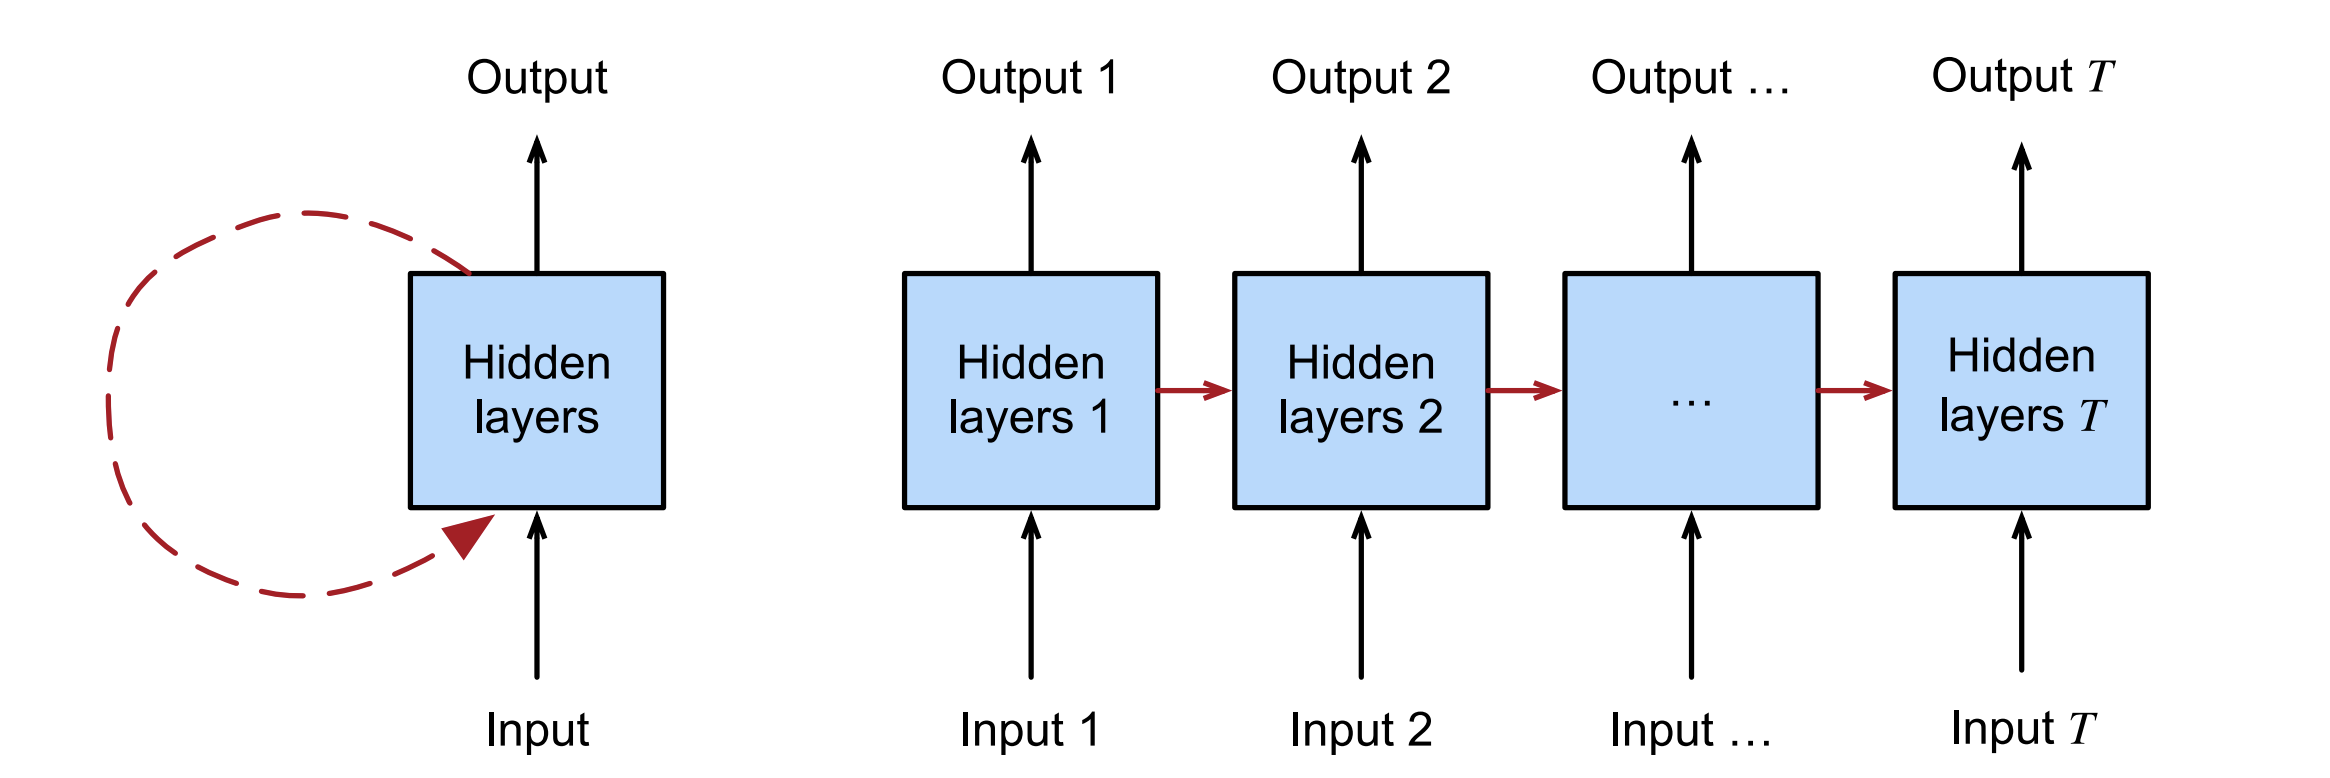
\includegraphics[width=0.7\textwidth]{rnn.png}
        \caption{\centering Diagram of a RNN at a single timestep $t$ (left) and unrolled in time between timesteps $0$ and $t$ (right)}
    \end{figure}

    To capture more information from the input sequences, RNNs can consist of multiple internal layers (shown in Figure BELOW), allowing them to learn higher-dimensional internal representations \citep{bengio-2009}. In this case, each layer $i$ retains its own internal state $h^{(i)}_t$, which is passed on to both the next layer of the network to compute its state $h^{(i+1)}_t$ (at the current input timestep) and reccurred back into itself at the subsequent timestep to compute the state $h^{(i)}_{t+1}$ \citep{zhang-2021}. 

    \begin{figure}[ht]
        \label{fig: deep-rnn}
        \centering
        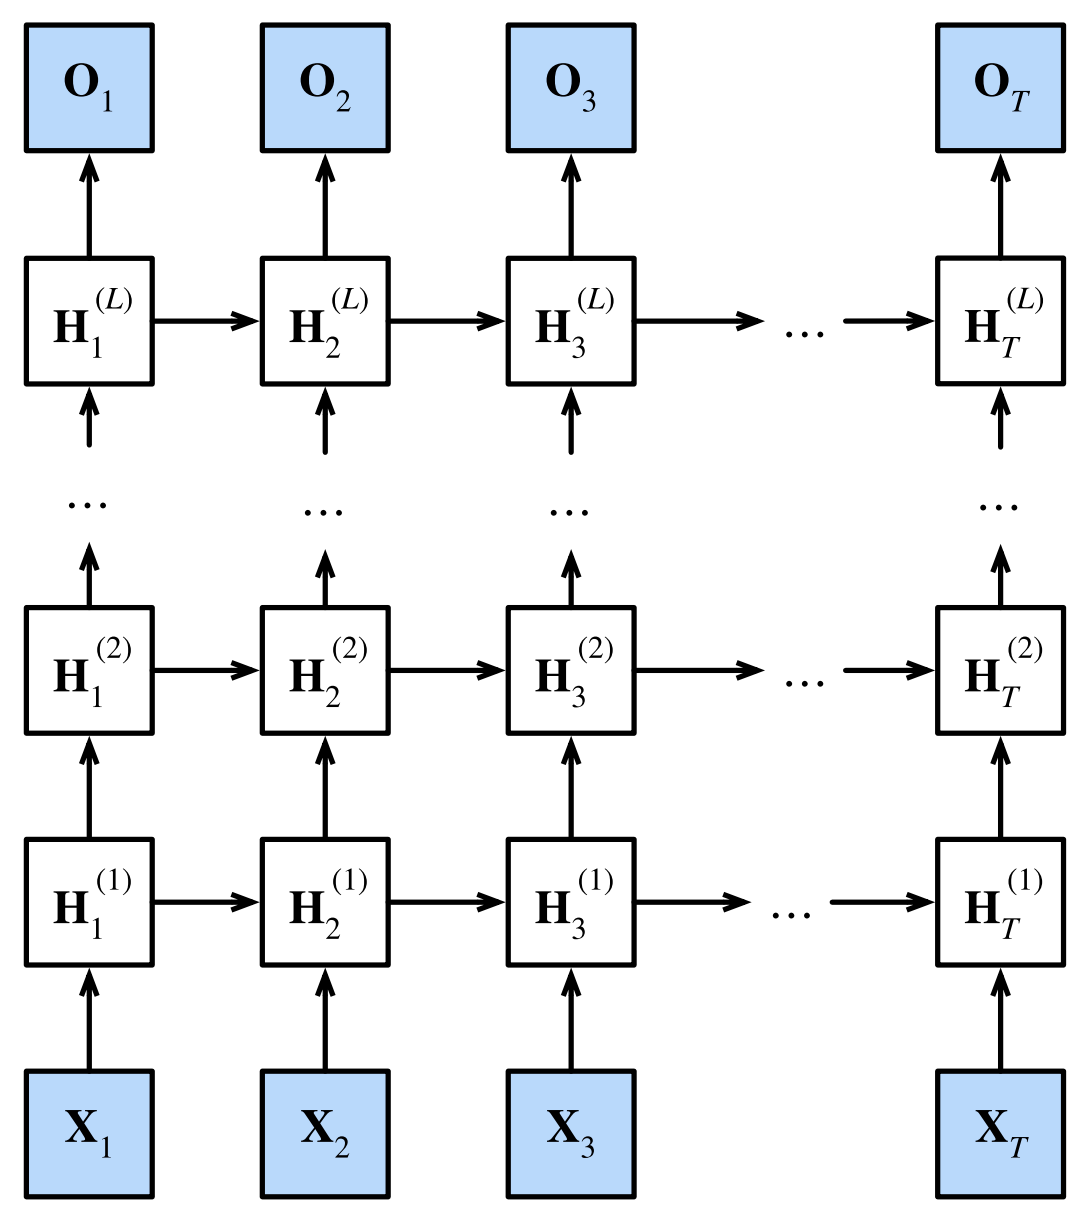
\includegraphics[width=0.4\textwidth]{deep-rnn.png}
        \caption{\centering Diagram of a multi-layer RNN (showing layers $1$ to $L$) with each layer unrolled in time between timesteps $1$ and $T$}
    \end{figure}


    \subsection{Training}

    Training of RNNs can be conducted through a similar backpropagation process to that used on traditional DNNs. This is done through computing the final output of the network on a given sequence (i.e. the output state at the final timestep) and evaluating the loss function between this and the true result, finding the total error of the RNN. The error is then propagated backwards through both the internal layers of the network and through time to the network state at each timestep of the input sequence---and hence is referred to as \emph{backpropagation through time} \citep{zhang-2021}. This allows the training procedure to adjust both the network parameters (i.e. weights $W$ and biases $b$) and the parameters $\theta^{(g)}$ of the state function $g$ determining how exactly the internal state $h^{(i)}_t$ is updated at each timestep.


    \subsection{Applications}

    Much recent research into sequence learning has exploited recurrent networks to conduct accurate modelling. In their review of the applications of RNNs within this domain, \citet{lipton-2015} explain how NLP tasks and time-series forecasting are the most common avenues explored by researchers utilising RNNs. These two areas have been extensively surveyed in literature; in their review of DL for NLP, described the rapidly increasing popularity of RNNs in recent years, highlighting language modelling, machine translation, speech recognition, and image captioning as major areas of recent process. They highlight the RNN model of \citet{karpathy-2015} for generating image descriptions---which significantly outperformed existing baselines---as a illustrative example of the benefits provided by this architecture. Additionally, \citet{hewamalage-2021} survey the current and future applications of RNNs for time series forecasting, highlighting the recent success of this model architecture at forecasting competitions, such as an RNN-based model by \citet{smyl-2020} winning The M4 Competition in 2019 with cutting-edge accuracy nearly $10\%$ greater than the utilised baseline \citep{makridakis-2020}.


    \section{Long Short-Term Memory}

    \subsection{The Issue with Recurrent Networks}

    The traditional RNN described above is incredibly effective at learning short-term dependencies within an input sequence, and exploiting these to make accurate predictions of subsequent values. In many cases, however, to understand the full context of a sequence longer-term dependencies need to be taken into account. Unfortunately, research into the effectiveness of recurrent networks by \citet{hochreiter-1991} and \citet{bengio-1994} has shown that RNNs cannot accurately capture or exploit long-term dependencies within sequences, as previous elements that are contextually relevant but were observed many timesteps ago can be forgotten prematurely. This issue is known as the short-term memory problem of RNNs, and is caused by the \emph{vanishing gradient problem} \citep{hochreiter-1991}. This issue is inherent to the backpropagation through time algorithm and the nature of recurrent variables. As demonstrated in Equation \ref{eq: rnn-state}, to calculate the value of a single recurrence involves multiplying by the weight matrix $W^{(g)}$: ignoring the bias and input element terms (as these aren't recurrent), we have $h_t = W^{(g)} \cdot h_{t-1}$. This poses a challenge when a recurrence is made over many steps, which is the case when evaluating the recurrent state function over many timesteps in a long sequence, as the same weight matrix is used over all recurrent state computations (shown in Equation \ref{eq: reccurent-weights} for a length $T$ sequence).

    \begin{align}
        \label{eq: reccurent-weights}
        h_T &= W^{(g)} \cdot W^{(g)} \cdot \ldots \cdot W^{(g)} \cdot h_0 \\
        &= (W^{(g)})^T \cdot h_0
    \end{align}

    Hence, the calculation is dependent on the computation of the weight matrix product $(W^{(g)})^T$; this means that if the parameters in the weight matrix are below one (i.e. we have $W^{(g)} < 1$) then the value of $(W^{(g)})^T$ will tend to zero with increasing sequence length $T$. This causes the gradient of the loss function with respect to the parameters $W^{(g)}$ to also tend to zero during backpropagation, meaning no significant updates are made to the values of $W^{(g)}$ when training on long sequences. Therefore, the gradient is said to \emph{vanish}, causing an inability of the network to learn dependencies over long sequences \citep{bengio-1994}.


    \subsection{Long Short-Term Memory Networks}

    Whilst several solutions to the vanishing gradient problem have been proposed---such as \emph{skip connections} and \emph{leaky recurrent units} \citep{pascanu-2012}---by far the most widespread approach is the use of \emph{Long Short-Term Memory} (LSTM), presented by \citet{hochreiter-1997}. An LSTM network is a RNN that uses multiple internal states and parameter matrices to mitigate the vanishing gradient problem and model both short-term and long-term dependencies within sequences. Similarly to an RNN, this architecture contains a core network consistent of one or more layers---where each layer is a distinct LSTM cell---and information is passed both between these cells (from the input to the output layer of the network) and between cell and and itself at the next timestep (reccuring the output at time $t-1$ to be input at time $t$). However, instead of the single recurrent state $h_t$ of the simple RNN, the LSTM contains two: a short-term memory state $h_t$ (analagous to that of a RNN) and long-term memory state $c_t$. This long-term state $c_t$ is used to retain information from far back in the input sequence, adding and forgetting relevant knowledge as the context of the sequence changes. 

    \begin{figure}[ht]
        \label{fig: lstm}
        \centering
        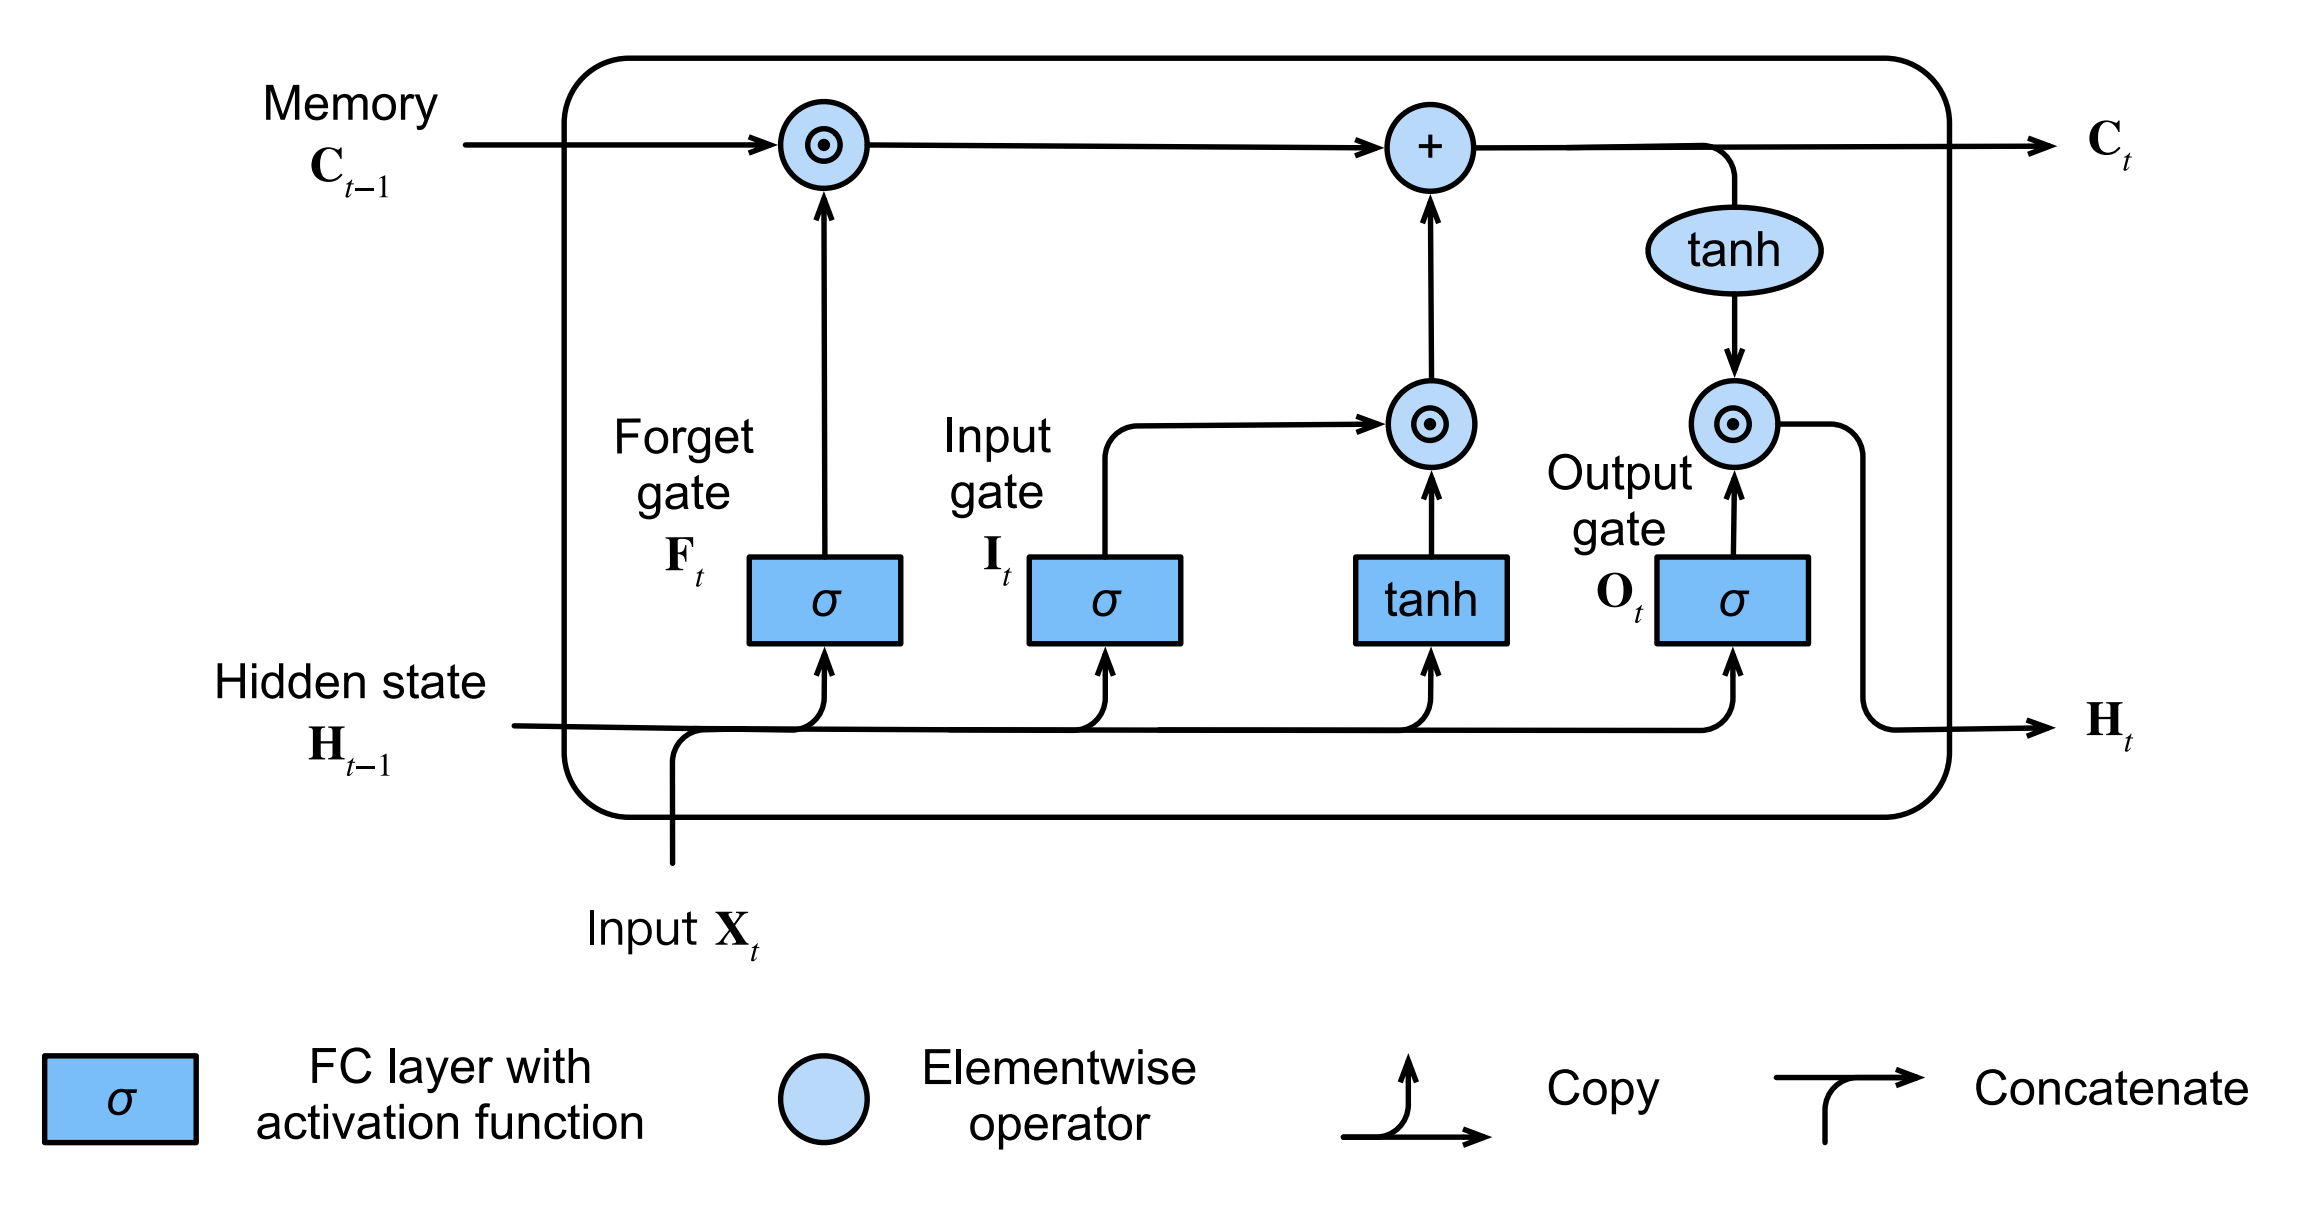
\includegraphics[width=0.7\textwidth]{lstm.png}
        \caption{\centering Diagram of a the arrangement of logical gates within a LSTM cell}
    \end{figure}

    At each timestep, the preceding long-term state $c_{t-1}$ is input into the LSTM cell (alongside the current sequence element $x_t$) to compute the new state $c_t$. These updates are achieved through several logical \emph{gates} within the network (between each cell and timestep). Firstly, the \emph{forget gate} is used to decide what information to discard from the previous state $c_{t-1}$. The previous short-term state $h_{t-1}$ and input element $x_t$ are multiplied with the forget gate's weight matrices $W^{(F)}$ and $U^{(F)}$ and added to its bias $b^{(F)}$, the result of which is passed through the \emph{sigmoid} activation function to produce the intermediate state value $\tilde{c}^{(F)}_t$, shown in Equation \ref{eq: forget-gate} \citep{zhang-2021}.

    \begin{equation}
        \label{eq: forget-gate}
        \tilde{c}^{(F)}_t = \sigma( W^{(F)} \cdot h_{t-1} + U^{(F)} \cdot x_t + b^{(F)} )
    \end{equation}

    Secondly, when new relevant information is seen in the input sequence, the \emph{input gate} is used to add it to the long-term memory state $c_t$. This process similarly uses the short-term state $h_{t-1}$ and current input $x_t$, but evaluates both a sigmoid and \emph{hyperbolic tangent} activation function in parallel on these inputs to decide both which values of $c_{t-1}$ must be updated (through the sigmoid evaluation) and by how much (the tangent evaluation). The result of these two operations are then multiplied together to give the second intermediate state value $\tilde{c}^{(I)}_t$, shown in Equation \ref{eq: input-gate} \citep{zhang-2021}.

    \begin{align}
        \label{eq: input-gate}
        (\tilde{c}^{(I)}_t)_{\sigma} &= \sigma( W^{(I,0)} \cdot h_{t-1} + U^{(I,0)} \cdot x_t + b^{(I,0)} ) \\
        (\tilde{c}^{(I)}_t)_{\tanh} &= \tanh{( W^{(I,1)} \cdot h_{t-1} + U^{(I,1)} \cdot x_t + b^{(I,1)} )} \\
        \tilde{c}^{(I)}_t &= (\tilde{c}^{(I)}_t)_{\sigma} \cdot (\tilde{c}^{(I)}_t)_{\tanh}
    \end{align}

    Both intermediate state values $\tilde{c}^{(F)}_t$ and $\tilde{c}^{(I)}_t$ are combined to give the new updated long-term state $c_t$ (Equation \ref{eq: long-state}).

    \begin{equation}
        \label{eq: long-state}
        c_t = \tilde{c}^{(F)}_t \cdot c_{t-1} + \tilde{c}^{(I)}_t
    \end{equation}

    The third and final gate used by LSTMs is the \emph{output gate}, which decides what each cell outputs. This is used as both the short-term state $h_t$ and the final network output $y$. The output gate uses the newly computed long-term state $c_t$, input $x_t$, and previous short-term state $h{t-1}$; a biased weighted sum of $h^{t-1}$ and $x_t$ is computed and fed into the sigmoid function, which is then multiplied by the hyperbolic tangent function evaluated on $c_t$ (Equation \ref{eq: output-gate}). Similarly to within the input gate, the sigmoid evaluation determines the values of $h_{t-1}$ to be updated, and the tangent evaluation determines by how much \citep{zhang-2021}.

    \begin{align}
        \label{eq: output-gate}
        (h_t)_{\sigma} &= \sigma( W^{(O)} \cdot h_{t-1} + U^{(O)} \cdot x_t + b^{(O)} ) \\
        (h_t)_{\tanh} &= \tanh{( c_t )} \\
        h_t &= (h_t)_{\sigma} \cdot (h_t)_{\tanh}
    \end{align}

    This system of gates occurs in every LSTM cell, passing information from the input to output layer of the network at every timestep in the form of the short and long-term states. When the network reaches the final timestep, the short-term state is output as the final network output $y$; note, if the sequence modelling problem involves outputting a generated sequence of length $N$ (e.g. forecasting multiple future values of a time series), this is produced one element at a time over $N$ additional timesteps that take no input and output the value $y_i = h_{T+i}$.


    \subsection{Applications}

    Whilst reviewing modern RNN architectures, \citet{lipton-2015} note that most state-of-the-art applications within the field of sequence learning use a LSTM-based model. Similarly,  in their review of the applications of this architecture and its variants \citet{yu-2019} assert that ``almost all" important recent advancements in this domain have been facilitated by LSTMs. This is primarily due to the architecture's ability to accurately model both long and short-term dependencies in sequences; hence, such networks are largely used for the same sequence modelling problems as traditional RNNs. 

    Due to the superior accuracy provided by this architecture, one of the most common use cases of LSTMs for sequence learning is NLP. For example, in their exhaustive study of language modelling, \citet{jozefowicz-2016} found an LSTM-based network to provide the most competitive results in this field. Their work evaluated several ML models such as \emph{convolutional neural networks} and RNNs, finding that a large scale LSTM language model produced the best results, significantly improving state-of-the-art \emph{perplexity} (a commonly used NLP metric of prediction error) from $51.3$ to $30.0$ on the commonly used \emph{One Billion Word Benchmark} dataset \citep{chelba-2013}. Recently, LSTM models have been applied to even more complex tasks within the NLP space due to the ability to capture high-fidelity dependencies. This includes the work of \citet{saleh-2021} who used an LSTM-based DNN to detect hate speech in online content, producing an impressive \emph{F1-score} (the weighted average of a model's \emph{precision} and \emph{recall}) of $93\%$ on a composite dataset from multiple online hate speech repositories.

    Like other RNNs, LSTMs have also been widely used for time series forecasting. Due to the advantages provided by these networks' ability to model long-term dependencies, the benefits of LSTMs have been explored across an extensive spectrum of different time series applications. For example, \citet{shi-2022} recently compared the performance of a number of networks (including both traditional RNNs and LSTMs) for predicting Bejing air quality. They concluded that LSTMs generated more accurate predictions than simpler RNNs, and demonstrated their improved long-term memory by showing LSTMs outperform other networks even when the context window available to the model is small. Another popular area of time series forecasting in which LSTM networks are increasingly being used is in the prediction of financial markets, as it has been shown by studies such as \citet{li-2017} that LSTMs can accurately capture the complex dependencies within highly variable financial variables. The success of LSTMs within this domain has been widely shown across a variety of financial modelling tasks, such as forecasting commodity prices \citep{ly-2021}, stock market indices like the S\&P 500 \citep{fjellstrom-2022}, currency pairs on the Foreign Exchange \citep{qi-2021}, and the fluctuations of financial market risk \citep{du-2019}.


    \section{The Efficiency of Recurrent Networks}

    The use of RNNs and LSTMs has revolutionalised sequence learning, permitting models with cutting-edge accuracy across a spectrum of applications, including financial risk forecasting \citep{du-2019}. However, further research into recurrent architectures has shown that the sequential processing methods vital to their performance also make these models highly inefficient.


    \subsection{Memory and Energy Efficiency}

    The tradeoff between accuracy and efficiency within RNNs has been explored by several recent research papers aiming to reduce the complexity and energy consumption of these architectures. In their study of compression techniques for LSTM models, \citet{wang-2018} identify this conflict as a core limiting factor of RNNs restricting their use in resource-constrained domains. This is similarly identified by \citet{zarzycki-2021} in their exploration of LSTM-based predictors for chemical reactors; they concluded that whilst the number of parameters utilised by an LSTM was directly proportional to its modelling performance, higher complexity models inflicted a significant computational cost. 

    Numerous sources, such as \citet{cao-2017}, \citet{feliz-2021}, and \citet{zhang-2021}, have deduced that this inefficiency is directly caused by the sequential nature of RNNs. They assert that the many dependencies within LSTM cells---both between cells and to the input sequence---restrict the way in which these models can be trained and used. Specifically, cells in an LSTM network take input from both the input sequence and preceding cells; each cell in every network layer and on every sequence timestep receives both an input vector and two memory states. \citet{cao-2017} highlight that this introduces both temporal dependencies (between cell states at each timestep) and layerwise dependencies (between the output and input of each network layer). Both \citet{cao-2017} and \citet{feliz-2021} identify that these dependencies mean that LSTM training and inference cannot effectively exploit parallelisation, as the sequential dependencies mean many operations have to be computed serially. Thus, these networks cannot fully take advantage of the computational speedups provided by specialised hardware such as \emph{Graphics Processing Units} (GPUs) and \emph{Tensor Processing Units} (TPU) that have been effectively used to parallelise other DNNs, making training long and energy-intensive \citep{zhang-2021b}.

    These explorations have also quantified the large memory requirements of complex recurrent networks. \citet{feliz-2021} concluded that accessing memory to fetch the parameters of an RNN is the main source of energy consumption during training. Similarly, \citet{cao-2017} found that larger models with more layers take more time (and energy) to load their parameters on each computational pass through the network. Because of this, the memory bandwidth (the speed at which data is sent to the processor) required for evaluating operations becomes a bottleneck to compute speed. Furthermore, \citet{zhang-2021} identify that the large intermediate values used between computations inside each LSTM cell (typically stored in a high-bit representation to maintain accuracy) require large amounts of memory to store, and expend significant energy to compute with.


    \subsection{Efficient Adaptations to Recurrent Networks}

    Several researchers have proposed methods for improving the efficiency of RNNs, typically through reducing memory requirements by either minimising the number of model parameters, compressing the network after training, or reducing the bit-size of variables. A notable exception to this trend is the language model of \citet{li-2016}, who suggested that training speed can be increased by reducing the number of possible network inputs. \citet{li-2016} showed that reducing the vocabulary of their RNN-based model decreased the required network size by a factor of $40--100$, decreasing training time by a factor of $2$. 

    Most commonly, training time, memory, and energy requirements can be reduced by shrinking an RNN's parameter set. The LSTM-based implementations of \citet{wang-2018} and \citet{chen-2022} achieve this through compressing the network; \citet{wang-2018} propose a structured compression technique that shrinks the necessary size of weight matrices, reducing the computational complexity of evaluating passes through the LSTM and decreasing the number of memory accesses required. This approach improved the model's energy efficiency by a factor of $33.5$ (compared to a state-of-the-art LSTM) whilst only inflicting a small accuracy drop. Similarly, \citet{chen-2022} implement a compact LSTM model, designed for the low resource requirements of medical sensors; they reduced the number of bits required to store variables, minimising memory constraints and simplifying expensive multiplications. Their network reduced power consumption by $56\%$ and the required circuit area of the specialised chip used by $54\%$ (compared to a typical 16-bit implementation).

    \citet{feliz-2021} extend the work of \citet{chen-2022} in reducing the complexity of calculations by lowering the precision of bit-representations. This approach utilised an additional policy network to identify instances within each network pass where the output of individual neurons doesn't significantly change between consecutive evaluations. If the policy network predicted only a minute change, the current output is cached and reused as the output of the next calculation, saving the need to evaluate the next computation. \citet{feliz-2021} found that this technique avoided over $24\%$ of computations, produced an average reduction in energy consumption of $18.5\%$, and reduced training time by a factor of $1.35$. Additionally, the policy network was used to dynamically select the bit-size of variables to maintain a compromise between accuracy and efficiency. This adaptation resulted in $57\%$ of computations being evaluated through a smaller representation, providing a further $19\%$ average energy saving and $1.46$ times training speedup.

    These results demonstrate that whilst RNNs are expensive in terms of memory and energy, several research directions have been proposed to mitigate this. The conclusions drawn show promise for improving the efficiency of RNNs and LSTMs, however, this research largely focuses on improving efficiency for specialised applications and hardware. Hence, further work in this field is required to demonstrate the general applicability of these adaptations to improving the efficiency of RNNs, especially within high-performance applications such as those in finance.


    \section{Financial Risk Modelling}

    Predicting stock price movements is a common example of sequence-to-sequence modelling that has received great attention within the field of deep learning for finance, with numerous reviews extensively exploring the area (such as \citet{sezer-2019} and \citet{jiang-2021}) and innovative approaches continually pushing the boundaries of prediction accuracy (e.g. the recent combination of deep learning and sentiment analysis by \citet{darapaneni-2022} for predicting stock price movements). Despite this plethora of research, it is still a challenging task to accurately model price movements in real financial markets due to the complexity of financial systems, non-linear relationships between financial variables, and high-frequency variations in values \citep{timmermann-2004}.


    \subsection{Forecasting Financial Risk}

    The challenges associated with market price prediction mean that within the finance industry a more helpful use case of sequence-to-sequence modelling is forecasting financial risk. In their white paper explaining the applications and benefits of ML for financial modelling, \citet{laplante-2019} exemplify this sentiment, asserting that ANNs provide the most utility for highlighting potential risks, not explicitly modelling variable movements. In fact, a recent survey of financial professionals by \citet{chartis-2019} found that $70\%$ of respondents use ML tools in the financial risk sector, majoritively for analysing ``market risk for the trading book" ($51\%$ of respondents) and ``market risk for the banking book" ($44\%$). This trend is echoed by \citet{peng-2021} in their review of Fintech, DL, and financial risk; they assert that modelling risk is currently in high demand due to the large fluctuations, uncertainty, and high volatility exhibited in financial markets, making risk an important consideration when making financial decisions. Furthermore, \citet{mashrur-2020} highlight that financial market risk typically exhibits identifiable trends as risk patterns reoccur in cycles, facilitating accurate modelling based upon historical data.

    For these reasons, modelling financial market risk is a popular application of DL. This typically involves the development of statistical models to forecast trends within different risk measures such as \emph{value-at-risk} (VaR) and \emph{volatility} \citep{peng-2021}. VaR estimates the value an asset is likely to lose over a given time period, to a specified confidence level, returning a value that indicates the maximum expected loss over that period at that confidence level. This metric has long been considered a valuable method of measuring market risk, with a vast spectrum of research covering its computation and use \citep{khindanova-2000}. Furthermore, studies such as that of \citet{sun-2009} have shown that ANNs provide superior forecasting of VaR than other models; this has established VaR popular choice for recent DL models aiming to forecast market risk using DNNs. For example, \citet{du-2019} proposed an RNN-based model for estimating VaR, showing that this approach provides a flexible architecture and improved prediction accuracy.

    Financial market volatility is also an important risk measure that is often forecast within academic research and the finance industry. Volatility can be defined as the scale of fluctuations in the pricing of an asset within a financial market over time and is intrinsically related to the risk associated with that asset \citep{cavalcante-2016}. \citet{cavalcante-2016} assert that this is a vital measure to financial analysis, as it is a key indicator of the state of many economic and external factors that affect financial markets (such as investor sentiment and political conditions). This is because changes to these factors directly affect the volatility of a market; for instance, in times of economic crisis or political instability, volatility tends to rise, meaning large price variations of assets are likely, and the market is considered high risk \citep{sezer-2019}. Because of this relationship between volatility and risk, \citet{tino-2001} highlight that volatility changes are typically used as buy and sell signals to investors, and \citet{ge-2022} assert market volatility dictates many decisions of market players; hence, forecasting market volatility is a popular modelling domain. In fact, whilst analysing models for the financial derivatives market, \citet{ozbayoglu-2020} found that most research into ML and DL-based modelling in this field either focuses on pricing or volatility estimation. This popularity is further demonstrated through the plethora of academic reviews specifically surveying this field, such as those by \citet{poon-2003} and \citet{ge-2022}, and the spectrum of recently proposed DNN-based forecasting models.

    \subsection{Measures of Volatility}

    The review of \citet{ge-2022} and recent exploration of volatility modelling by \citet{tino-2001} both provide comprehensive overviews of the most commonly used measures to quantify volatility measures: \emph{historical volatility}, \emph{realised volatility}, and \emph{implied volatility}. Due to their relative simplicity, these three metrics have been extensively explored in literature and their ability to be forecast demonstrated. Each of these measures calculates a slightly different version of volatility. Implied volatility (IV) is computed given a specific option price, computing the expected volatility associated with that price; whereas, realised volatility (RV) is a measure computed directly from the price movements of a market and hence is the volatility actually realised in the underlying financial market. Historical volatility (HV) is a type of realised volatility, which computes the volatility over a preceding time period based upon market closing prices; it is the opposite of \emph{future realised volatility}, which is the forecast value realised volatility is expected to take in the future \citep{busch-2011}.

    Due to the differences in what these measures represent, each is computed in a slightly different way. Since IV represents an expectation of volatility, it cannot be computed directly from financial market data; instead, IV is estimated through an option pricing model such as the \emph{Black-Scholes model} \citep{black-1973}. Options models are typically used to estimate the price of an option (a financial contract between buyers and sellers) under the current market conditions \citep{wu-2015}. When inverted, these models can additionally be used to compute IV by inputting a given option price \citep{tino-2001}. On the contrary, RV is computed directly from market price movements over a time window $\tau_1 \to \tau_2$ \citep{ge-2022}. This measure is typically calculated as variation in the logarithmic returns $r_t$ of an asset (Equation \ref{eq: return}) over the specified time period. Most commonly, this time window covers returns observed in the past, which is the HV of that period. When surveying various volatility measures, \citet{ge-2022} found HV to be the most popular, primarily because it provides an intuitive metric that is simple to compute. The most common method of computing HV is to approximate the volatility $V_t$ over the $N$ values over the interval $t \colon \tau_1 \to \tau_2$ as the standard deviation of logarithmic returns between these times; this is shown in Equation \ref{eq: hv1}, where $\mu(\tau_1, \tau_2)$ is the mean return over the time interval \citep{ge-2022}. This method of computing HV is used across a wide range of applications within volatility modelling, such as the ANN-based model of \citet{lahmiri-2017} that forecasts the volatilities of the exchange rates between currency pairs.

    \begin{equation}
        \label{eq: return}
        r_t = \log\Big(\frac{c_t}{c_{t-1}}\Big)
    \end{equation}

    \begin{equation}
        \label{eq: hv1}
        V_t = \sqrt{ \frac{1}{N} \sum_{t' = \tau_1}^{\tau_2} \big( r_{t'} - \mu(\tau_1, \tau_2) \big)^2 }
    \end{equation}

    Whilst this is the most commonly referenced method of computing HV, a spectrum of different formulae have been proposed. For example, \citet{tino-2001} computed HV as an exponentially weighted average (by weighting factor $\alpha \in [0, 1]$) of the square of logarithmic returns over the time window (Equation \ref{eq: hv2}). 

    \begin{equation}
        \label{eq: hv2}
        V_t = (1 - \alpha) \sum_{t' = \tau_1}^{\tau_2} \alpha^{\tau_2 - t'} r_{t'}^2
    \end{equation}

    In their review of 35 volatility forecasting ANNs, \citet{ge-2022} found HV was the most popular metric, constituting $71\%$ of research papers; this was followed by other RV measures ($17\%$), and finally IV ($9\%$). Additionally, \citet{ge-2022} explored the most common domains for forecasting volatility, finding the S\&P 500 market to be the most popular (accounting for 12 out of the 35 research papers), primarily due to its accessibility; the price of oil (7 papers) and metal (6 papers) were also found to be common modelling applications. However, a vast spectrum of models have been developed outside of these domains; for instance, \citet{ge-2022} also explored the use of IV, RV, and HV within the context of stocks, bonds, and other financial indices. Hence, the selection of a volatility measure is typically a domain-specific choice, based upon the different benefits and drawbacks associated with each metric. For example, IV has been seeing increased adoption from institutional investors, hedge funds, and banks \citep{neftci-2008}, and is used to define major volatility indices such as the \emph{Chicago Board Options Exchange's Volatility Index} (VIX). However, due to its reliance upon an options pricing model, IV requires options data, and hence cannot be used in other domains; furthermore, it exhibits the \emph{volatility smile}---where near-identical option prices can result in highly different volatility levels---and tends to output higher volatility than other measures. There are also challenges associated with RV and HV; whilst RV has been shown to tend towards an estimate indistinguishable from the latent volatility \citep{andersen-2001}, this accuracy requires data with a high sampling frequency. Additionally, several issues unanimously encompass all volatility estimates, including price irregularities at the tail-ends of return distributions (discussed in detail by \citet{ozbayoglu-2020}) and the complex dependencies and transient relationships between financial variables \citep{timmermann-2004}.


    \subsection{Forecasting Financial Volatility}

    Due to the utility of modelling financial risk, forecasting market volatility has become a popular domain within both financial computing research (such as within the survey of \citet{ozbayoglu-2020}) and the finance industry (shown through the statistics gathered by \citet{chartis-2019}). Furthermore, \citet{ge-2022} demonstrates this is a global trend, discovering that the 35 research papers they surveyed were derived from 11 different countries (including the US, UK, Germany, and China).

    Traditionally, financial institutions and researchers have exploited \emph{generalised autoregressive conditional heteroscedasticity} (GARCH) models to forecast volatility. GARCH models have been shown to be accurate and reliable, with research such as that of \citet{lahmiri-2017} demonstrating the ability of these systems to capture the characteristics of financial time series. These models calculate the volatility of a market from a series of logarithmic returns, approximating the volatility $V_t$ at time $t$ as the conditional variance $\sigma_{t}^2$ of returns over a specified time period. Early work in this field by \citet{akgiray-1989} showed that GARCH models managed to fit training data (a time series of stock returns) and forecast volatility at future timesteps more accurately than similar models in its class. Similar studies, such as that of \citet{hansen-2005}, have also demonstrated the impressive forecasting accuracy of GARCH models within the foreign exchange market. Additionally, GARCH models have been shown to accurately determine clusters of high and low volatility, which gives a good insight into the short-term risk exhibited in a market as high volatility is typically followed by high volatility, and vice versa \citep{arum-2019}. Largely because of this accuracy, GARCH has become one of the most frequently utilised methods of estimating the volatility of financial time series \citep{cheng-2003}. Even despite modern methods, this model is still a popular choice, often being used as a baseline to judge the performance of newly proposed volatility forecasting models; for example, \citet{rodikov-2022} used GARCH to contextualise the results of their DNN-based system. The calculations inherent to GARCH have also recently been used in several hybrid models to complement the computation of volatility within a larger system. In fact, the survey of volatility forecasting models by \citet{ge-2022} found that of the 35 papers reviewed, 14 focussed upon hybrid models; of these, they found GARCH to be the biggest contributor. \citet{tino-2001} similarly discuss the prevalence of hybrid models, asserting that they combine the predictive performance of complex models with the robustness of simple methods (such as GARCH) for dealing with non-stationary data.


    \subsection{Deep Learning for Volatility Forecasting}

    Whist traditional forecasting methods have been shown to produce accurate estimations of the risk of financial markets, a significant amount of recent work has focussed on applying DL-based modelling to this domain; for example, \citet{chartis-2019} found that $70\%$ of financial institutions use ML for risk analysis and forecasting, most commonly for ``market risk". This has become a popular domain within computational finance research. Such research has included the DNN of \citet{kim-2020} for forecasting the profitability and operational risk of the trading behaviour of retail investors in the stock market, and \citet{groth-2011} who analysed unstructured text data to identify news relating to corporate disclosures that are likely to cause abnormal volatility levels in the stock market. Forecasting the VaR of assets is also a popular application of DL within financial risk, such as the RNN-based approach of \citet{arimond-2020}. In fact, in their analysis of the intra-day risk of the German stock market, \citet{sun-2009} proved that ANNs provide superior forecasting accuracy of VaR compared to other traditional methods. This improved accuracy is one of the core reasons why DL is being increasingly adopted within financial risk, as \citet{chartis-2019} found that $44\%$ of financial firms cite ``greater accuracy of process and analysis" as the motivation behind using ML methods.

    Volatility forecasting is also becoming a popular application of DL; through analysing the publication rate of research papers in 2018, \citet{sezer-2019} found that volatility forecasting was in the top five uses of DL within financial research. Additionally, in their review of ML-based volatility models, \citet{ge-2022} asserted that almost all recent work on forecasting financial volatility relied on ML and DL methods, largely due to their improved accuracy and ability to fit complex time series. This performance improvement has been exemplified through several extended studies; for example, \citet{zhang-2022} found that ANNs can model the strong and stable commonality in intra-day RV to produce better forecasting performance that takes advantage of the shared features between financial variables. These results demonstrated how DNNs are superior at handling complex interactions and dependencies between financial variables, as their high dimensionality allows them to act as better function approximators.

    Several studies have compared the performance of DL models to traditional methods. Through an evaluation of volatility forecasting models over 23 different stocks, \citet{rahimikia-2020} found that DL gives stronger forecasting power than autoregressive methods such as GARCH. \citet{rodikov-2022} drew a similar conclusion, finding that an LSTM-based model could generate a higher test accuracy than other well-known models. They also found that RNN architectures were effective at estimating financial market variables like volatility as they do not need to know the parameters of the underlying distribution of the variable being forecast. This is different from models such as GARCH, which uses \emph{maximum likelihood estimation} to approximate the parameters of the return and variance functions of the market. Furthermore, \citet{tino-2001} assert that GARCH has been shown not to be able to facilitate notable profits for investors, whereas RNN-based models show promise in facilitating a statistically significant profit for market players using them within their trading strategy. 

    Whilst some researchers opt for alternative architectures (such as the CNN-based model of \citet{chen-2018}), the improved accuracy and potential profit offered by RNNs and LSTMs have established them as a core focus of DL models for volatility forecasting. In their survey of 35 research papers, \citet{ge-2022} found that 9 out of the 21 pure models utilised an RNN, as these networks are a natural fit for time series data. This research typically explores the use of RNNs for forecasting realised volatility within the S\&P 500 market. For instance, \citet{bucci-2020} showed that RNNs outperform all other traditional methods for forecasting RV over S\&P 500 data. Their experimentation demonstrated the ability of an LSTM to capture long-term dependencies within the financial time series, which made this architecture more accurate at forecasting during highly volatile periods. Additionally, \citet{xiong-2016} incorporated Google domestic trend data into their RNN-based model for the S\&P 500, finding that RNNs are more robust against noise in the time series data. Hybrid models that combine RNNs within traditional methods have also been explored in literature, with \citet{ge-2022} finding that 14 of the 35 surveyed papers implemented a composite system. Most commonly, this approach uses a GARCH model to aid the DNN's computation of volatility; for example, \citet{kim-2018} combined an LSTM with GARCH to generate highly accurate predictions of RV over the South Korean stock market.

    Hence, it is clear that the use of DL (in particular RNNs and LSTMs) is an expanding field within financial volatility forecasting. This is primarily due to the increased forecasting accuracy provided by DNNs, as these models have been shown to produce class-leading performance across markets (such as the S\&P 500) and volatility metrics (most notably RV). 


    \section{Green AI}

    Complex DL-based systems are seeing increased adoption across a variety of modelling domains in finance and further afield, primarily due to their superior accuracy. However, many of these implementations ignore the efficiency concerns associated with DL, such as the memory and energy inefficiency of recurrent networks. The ignorant use of these resource-hungry models (dubbed Red AI by \citet{schwartz-2019}) inflict large ESG costs, as their extreme computational load generates thousands of pounds of carbon emissions over training \citep{strubell-2019}, and limits who can research and employ within high-performance ML systems \citep{bender-2021}. These environmental and social impacts have spurred recent attention around Green AI, where DL energy and data-efficient models are developed, motivated by reducing resource requirements, mitigating environmental cost, and benefiting the inclusivity of ML \citep{schwartz-2019}.


    \subsection{Quantifying the Energy Efficiency of Deep Learning}

    As a simple initial approach to mitigating the ESG cost of DL, many proponents of Green AI suggest that all new research papers on cutting-edge DL models should report the training time and resource requirements of their DNNs. \citet{strubell-2019} assert that this should allow future work looking to utilise existing methods to conduct a cost-benefit analysis based upon the resources required to implement such a model. In their analysis of 60 DL research papers, \citet{schwartz-2019} found that $90\%$ of papers in the ACL Anthology, $80\%$ of those in the NeurIPS conference, and $75\%$ in the CVPR conference cited accuracy improvements as the main contribution of their work, with only $10\%$ of ACL papers and $20\%$ of CVPR papers contributing a new efficiency result. \citet{schwartz-2019} argue that this demonstrates the lack of reporting surrounding the energy and data efficiency of DL models, highlighting that describing performance contextually with respect to training budgets improves both the sustainability and inclusivity of this work (allowing future work to be compared despite fewer training resources).

    Despite the consensus on the importance of reporting the resource requirements of these systems, a ubiquitous hardware-independent measure of the computational cost of a DL model has yet to be firmly agreed upon. \citet{schwartz-2019} describe how the expense $Cost(R)$ of processing the result $R$ using a DNN is proportional to the cost of processing a single instance $I$, the size $D$ of the training dataset, and the number of hyperparameters $H$ that require tuning (Equation \ref{eq: cost-r}). They survey several proposed metrics for quantifying this cost, including runtime, parameter count, electricity usage, and carbon emissions; however, they highlight that each of these poses its own challenges, such as the hardware-dependent nature of electricity usage and difficulty in measuring the exact carbon emissions produced by a program. \citet{schwartz-2019} conclude that reporting the total number of \emph{floating-point operations} (FLOPs) to generate the result is the most reliable way to quantify the computational cost, and hence energy efficiency, of a system. This count provides several advantages over alternative metrics: it accurately reports the computational work done by a system, is correlated to runtime (through considering work per time step), and has been successfully used to quantify the energy footprint of ANNs \citep{veniat-2018}.

    \begin{equation}
        \label{eq: cost-r}
        Cost(R) = I \cdot D \cdot H
    \end{equation}

    \citet{schwartz-2019} use the competing models ResNet (he-2015) and ResNeXt (xie-2017) to exemplify how reporting FLOPs can contextualise performance advancements with model efficiency: whilst ResNeXt provided a $0.5\%$ accuracy boost over the \emph{ImageNet} dataset (becoming 2017's leading \emph{ImageNet top-1 accuracy} score), it required $35\%$ more FLOPs. However, \citet{schwartz-2019} note that using FLOP count as an efficiency metric is not without its own limitations; most importantly, FLOP doesn't always exactly correlate with runtime or energy consumption, as it does not take into account auxiliary communication or memory costs. \citet{amodei-2018} echo these benefits of reporting FLOP; however, they highlight that computing the FLOP count of a program is not always trivial. They suggest that in the absence of being able to directly compute the FLOPs of a given DL model, its computational load can be approximated through its GPU utilisation over training; this calculation is demonstrated in Equation \ref{eq: cost-t}, where the computational cost of training $Cost(T)$ in \emph{petaFLOP/s-days} (pfs-days) is given by the product of the number of GPUs used $N_{gpu}$, the processing power per GPU in FLOP/s $P_{GPU}$, the training time in days $T_{days}$, and the estimated average utilisation of these GPUs $U$ (typically taken as $33\%$). To exemplify this approximation, \citet{amodei-2018} calculated that whilst 2012's leading image classifier AlexNet \citep{krizhevsky-2012} had an approximate computational cost of $0.0058$pfs-days, five years later the innovative DNN \emph{Xception} \citep{chollet-2017} had a cost of $5.0$pfs-days (an increase by a factor of $862$).

    \begin{equation}
        \label{eq: cost-t}
        Cost(T) = N_{gpu} \cdot P_{gpu} \cdot T_{days} \cdot U
    \end{equation}

    Further work has attempted to explicitly quantify the carbon emissions associated with ML systems, despite the challenges of this metric identified by \citet{schwartz-2019}, who state that emissions are highly dependent on local electricity infrastructures and hence are often hard to compare between models and regions. For example, \citet{lacoste-2019} propose a \emph{Machine Learning Emissions Calculator} that computes the $CO_2$-equivalents ($CO_2$-eq) of an ML system, measuring the environmental detriment caused by the energy expended training a given model. They assert that despite its complexity to compute, measuring $CO_2$-eq is highly beneficial as it gives a direct insight into the emissions we are trying to minimise.

    This work demonstrates that quantifying the computational, energy, and carbon cost of existing and newly proposed DNNs is an expanding field within DL research and Green AI, solidifying quantification methods as a vital first step to raising awareness about the ESG impacts of DL, and promoting the use of energy-efficient models.


    \subsection{Efficient Neural Network Architectures}

    Once the ESG impact of DNNs has been thoroughly quantified, this information must be taken into account by developers to ensure that new models are developed efficiently. As \citet{schwartz-2019} identify, the cost associated with generating a result from a DNN is proportional to that of processing a single instance $I$. Hence, much research into Green AI has focussed on how the architecture of DNNs can be redesigned to minimise computational complexity and the energy expended to process data instances. 


    \subsubsection{Shrinking Model Sizes}

    Smaller neural networks expend less energy to generate a result, as fewer layers mean fewer computations and memory accesses. For this reason, a significant proportion of Green AI research focuses on developing \emph{compact models}, either through reducing the number of layers within a given ANN or \emph{pruning} its parameter set. In an exploration of the carbon footprint of ML, \citet{lottick-2019} evaluated the energy budget and carbon emissions of increasingly large ANNs. Interestingly, their research showed that whilst increasing the number of layers within an MLP increases its energy consumption, it does not generate a consistent improvement in accuracy, and could even degrade performance. Hence, \citet{lottick-2019} assert that accurate models do not have to be complex, and compact DNNs offer significant promise in generating impressive performance whilst reducing the energy expenditure.

    Early work into ANNs and DNNs focussed on \emph{fully connected networks} (FCNs) that required incredibly large parameter sets and consumed extreme amounts of energy to process data. In an attempt to reduce the cost of such models as networks got deeper, \citet{han-2015} proposed \emph{network pruning} for generating efficient ANN architectures. This method took a pre-trained ANN and allocated an importance score to each channel weight, quantifying its significance to the network's performance. Redundant channels with a score below a given threshold were identified and removed from the ANN, producing a model that maintained accuracy but had a reduced computational and memory cost. \citet{han-2015} demonstrated their pruning technique on AlexNet, producing a $9.1$ times reduction in parameter count from $61$ to $6.7$ million without any accuracy reduction. This impressive result demonstrated the promise of compact models with lower resource requirements, inspiring a spectrum of new research into pruning. For example, \citet{iandola-2016} used a similar pruning technique to \citet{han-2015} to produce an efficient ANN SqueezeNet for deployment in low-memory embedded systems; their model surpassed AlexNet accuracy whilst reducing the parameter set size by a factor of $50$. This dramatic reduction further demonstrated the utility of parameter pruning to applications with limited resources. Additionally, parameter pruning has been applied to RNNs---such as the pruned RNN-based translation model of \citet{see-2016} and compact network of \citet{narang-2017}---producing effective models for sequence learning with lower computational costs.


    \subsubsection{Quantisation and Efficient Variable Representations}

    Due to the publicity surrounding the record-setting performance of complex DNNs, these models are alluring tools for industry players looking to upgrade their workflows—notably \citet{chartis-2019} found that $44\%$ of financial firms cited ``greater accuracy" as the motivation behind adopting ML. However, in many cases, the upper echelons of performance are neither necessary nor beneficial for industrial applications; \citet{kumar-2020} highlight that in resource-constrained applications such as on mobile devices, state-of-the-art DNNs are not feasible as they would quickly engulf the limited power and memory resources. For this reason, Green AI researchers have begun to explore how accuracy-efficiency tradeoffs can be made that produce significant decreases in the energetic cost of DNNs by inflicting slight accuracy drops.

    Much of this research, explored in surveys such as those of \citet{xu-2021} and \citet{cai-2022}, has focussed on decreasing computation and memory costs by using lower precision representations of variables and parameters. Typically this is implemented through \emph{quantisation}, where the value of each variable is mapped to discrete quantisation levels that require fewer bits to store. \citet{xu-2021} divide these quantisation methods into two classes: \emph{deterministic quantisation} and \emph{stochastic quantisation}. The former computes an explicit, pre-determined mapping between original values and their low-bit quantised counterparts, whilst the latter selects the quantised value probabilistically; for example, \emph{random rounding} samples low-bit representations from a discrete distribution where each possible quantisation level has a given probability. Deterministic approaches range from \emph{uniform quantisation}, where floating-point numbers are mapped to their closest low-bit fixed-point representations, to \emph{clustering quantisation}, where parameters are clustered by value and replaced by the mean of their cluster \citep{xu-2021}. \citet{kumar-2020} demonstrate the performance of rounding quantisation by comparing the DNN-based approaches of \citet{courbariaux-2015} and \citet{judd-2016}. Namely, \emph{BinaryConnect} \citep{courbariaux-2015} implements an extreme quantisation approach, using only single-bit representations, but inflicts an accuracy drop of $19\%$; whereas, \emph{Stripes} \citep{judd-2016} reduce variable representations from 32 to 8-bits whilst maintaining an accuracy drop of only $1\%$. Hence, quantisation is an incredibly adaptable technique and can be widely used to decrease the computational cost of models contextually based on their desired accuracy-efficiency tradeoffs.

    These methods implement post-training quantisation, which improves the efficiency of models after they have been developed. Further research has explored quantisation-aware training, which aims to reduce the performance drop inflicted by quantisation by applying it at each training step. For example, \citet{fan-2020b} quantised parameters during training to produce a model that achieved an ImageNet top-1 accuracy score of $80.0\%$ (equivalent to 2017's highest accuracy model ResNeXt) using only $3.3$MB of memory (only $3\%$ of the memory required by ResNeXt). Furthermore, \citet{cai-2022} assert that this training process can be adapted even further to conduct \emph{low-bit training}, where parameters, activation values, and error gradients are all quantised. \emph{DoReFa-Net} \citep{zhou-2016} implemented such low-bit representations, using 1-bit parameters, 2-bit activations, and 6-bit gradients to boost training speed whilst generating an accuracy comparable to AlexNet using 32-bit representations. This demonstrates that quantisation and low-bit representations can be effectively used to produce models with significantly lower memory constraints and energy consumption. Research has also been conducted into quantisation for RNNs and LSTMs: \citet{hubara-2016} explored the effectiveness of quantising weights and activations within recurrent networks, whilst \citet{he-2016} proposed quantising LSTM gates. However, whilst investigating quantisation for RNNs, \citet{ott-2017} found that low-bit training was not ubiquitously effective at preserving accurate performance; thus, they concluded \emph{mixed-precision training} should be used for RNNs, where weight matrices are quantised but activation values retain higher bit representations.


    \subsection{Efficient Model Training}

    Whilst the efficiency of a DNN's architecture is essential to minimising the energy expended by each pass through the network, it is also important to minimise the total number of passes required by training. Hence, a significant amount of research within Green AI focuses on energy-efficient training algorithms that attempt to reduce the number of iterations necessary to train an accurate model.


    \subsubsection{Transfer Learning}

    Possibly the most common method of reducing the length of a DNN training phase is simply utilising a pre-trained model developed for another analogous task. This method, known as \emph{transfer learning}, is discussed by \citet{strubell-2019}, \citet{walsh-2021}, and \citet{schwartz-2019} in their explorations of Green AI. Specifically, transfer learning takes an existing pre-trained \emph{base model}, and tunes its parameters over a new training dataset that covers a new domain. Since the base model has already learned a general ability to complete a similar task, the new target model requires only a short, computationally-inexpensive retraining process, where the model is fine-tuned to accurately capture information from the new domain. Both \citet{strubell-2019} and \citet{walsh-2021} identify that transfer learning significantly reduces the resources required to train a DNN and allows their application within fields with only limited amounts of data. For example, \citet{wang-2020} used transfer learning to apply ResNet to the \emph{Stanford Dogs 120} dataset, a small collection of only 20,580 images, making it only $1.7\%$ of the size of the original ImageNet dataset (of 1.2 million images) used to train ResNet. The use of transfer learning allowed \citeauthor{wang-2020} to develop a model that had an accuracy $11.07\%$ greater than any other DNN developed for this data and reduced the required training iterations by a factor of $10$. This demonstrates that transfer learning is a simple but effective method for reducing the training cost of DNNs, which allows models to be developed for niche domains and minimises the energy required to train accurate ML models. Furthermore, the cost of training the original base model is effectively spread over all target models that utilise it, sharing out its computational cost. For this reason, \citet{schwartz-2019} advocate for more pre-trained models to be released publicly in an attempt to promote transfer learning and minimise the ESG impact of state-of-the-art DL models.


    \subsubsection{Initialisation}

    Instead of directly copying a base model, its parameter values can be used as a starting point from which training a new DNN can begin. This is an example of \emph{initialisation}, which is the process through which the initial values in a network's parameter set are chosen. This is an important part of training, as \citet{xu-2021} found that the rate of convergence of a network's parameters (towards the minimum of the loss function) heavily depends upon their initial values. Furthermore, \citet{hanin-2018} found that primitive techniques for initialising DNNs such as random initiation from a uniform or Gaussian distribution can often lead to slow training, or even result in parameter values never converging.

    Both \citet{hanin-2018} and \citet{xu-2021} evaluate alternative methods by which a network's parameters can be initialised. As described, this could be from an existing model trained over a base task, which is believed to improve generalisability and reduce training time. There are a number of varying ways in which this has been implemented; \emph{feature-based initialisation} assigns borrowed parameter values to a subset of the new DNN's parameters and keeps these fixed during training (improving generalisability), whereas \emph{fine-tuning-based initialisation} trains all new and borrowed parameters, providing greater specialisation. Alternatively, \emph{supervised initialisation} (commonly used for CNN architectures and NLP models) pre-trains the new DNN over similar datasets or for analogous tasks, then reuses these low-level representations as a starting point for training high-level features in the target task over the target dataset. For example, lin-2021 initially pre-trained their DNN-based language model as a general multilingual translator, before specifically applying the network to language pairs to translate between. \emph{Self-supervised initialisation} takes this concept further, allowing pre-training to be conducted without supervised data by learning general representations over unlabelled data (e.g. \emph{ELMo} by \citet{peters-2018}).

    Hence, this established research demonstrates the importance of selecting a suitable initialisation method when developing a new DNN based upon the chosen application and architecture, as the starting point of training can drastically reduce the time and energy expended to generate an accurate model.


    \subsubsection{Progressive Training}

    \emph{Progressive training} \citep{xu-2021}, also known as \emph{greedy layer-wise pre-training} \citep{xu-2018}, builds upon the aforementioned concept of building up a DNN through a combination of pre-training and tuning. This training procedure constructs a model sequentially layer-by-layer by iteratively adding a new layer and tuning its parameters. This builds up the DNN in a bottom-up approach, whereby the network first trains lower layers to accurately represent low-level features of the input, then trains higher layers based upon the learned parameters of the preceding layers (keeping the parameters of the previously added layers fixed). After the desired number of layers has been added, all parameters are unfixed and their values tuned in a concluding training phase. In theory, this reduces the computational cost of training a DNN, as training shallow, single-layer networks is significantly simpler and less resource intensive than training full, deep networks \citep{xu-2021}. Furthermore, \citet{xu-2021} assert that the parameters of later layers are optimised faster, as values are updated based on information already known about the features of the input (learned while training previous layers). This approach has been successfully used by implementations such as \citet{yang-2020} to radically speed up training. Specifically, \citet{yang-2020} reduced the total training time required by the language model BERT by over $110\%$ (from $85$ to $40$ hours) without degrading accuracy.

    Progressive training is typically implemented through one of two methods: \emph{supervised layer-wise pre-training} or \emph{unsupervised layer-wise pre-training}. Supervised approaches, such as that of \citet{ienco-2019}, train individual layers in a supervised manner, greedily optimising the performance of each. For instance, if building a forecasting model (such as the LSTM-based model of \citet{xu-2018}), each layer is independently trained to predict the future elements of a sequence. Starting by training a shallow network consisting of only an input layer, one hidden layer, and an output layer, the model iteratively gets deeper; this is achieved by first removing (and saving) the output layer, then fixing the values of all previously trained parameters, adding a new hidden layer, appending the saved output layer, and finally training the parameters of this new layer. Once a network of the desired depth has been constructed, the parameters of all layers are unfixed, and a short training round is conducted over the full network, where the parameters found during pre-training are used as a starting point for deducing the optimal global parameter set. 

    Unsupervised approaches, such as the implementations of \citet{xu-2018} and \citet{sagheer-2019}, train each additional layer as an \emph{auto-encoder}. Autoencoders are a type of ANN that learn to output a condensed or encoded representation of its input; they are trained in an unsupervised manner by simply minimising the difference between the input vector and the network's output vector \citep{pinaya-2019}. In unsupervised layer-wise pre-training, network layers are also built up iteratively. However, when it comes to training individual layers, each is trained as an unsupervised autoencoder, and hence learns to output a representation of the input vector it receives from its preceding layer (or the input layer in the case of the first hidden layer). This unsupervised learning is repeated over the entire pre-training process, to result in an autoencoder network of the desired depth \citep{sagheer-2019}. During the subsequent training process of the full network, the model is then repurposed to the desired task (e.g. forecasting sequence elements). Namely, the autoencoder output layer used during pre-training is discarded, and a new output layer for the desired task is appended. With all parameters unfixed, the network then undergoes training, starting from the parameter set found during pre-training, and optimising the network's performance in the chosen domain \citep{sagheer-2019}.

    Research into layer-wise pre-training commonly centres around improving the efficiency of training recurrent networks, as RNNs have been identified as one of the most sensitive architectures to parameter initialisation. Namely, \citet{xu-2018} highlighted that poor training initialisation of RNNs can cause parameters to converge to sub-optimal values, and \citet{ienco-2019} found poorly initialised networks resulted in models with weak generalisability. Fortunately, both supervised and unsupervised layer-wise pre-training have been shown to combat these issues. \citet{ienco-2019} showcase how supervised layer-wise pre-training can be used to produce an RNN-based sequence classifier that matched and exceeded the accuracy of comparable models in a number of applications. Both \citet{xu-2018} and \citet{sagheer-2019} demonstrate that unsupervised layer-wise pre-training is effective at improving training efficiency while preserving accuracy. By comparing LSTM models initialised with layer-wise pre-training to a simple randomised initialisation, \citet{xu-2018} exemplified the performance and efficiency benefits of this technique across a number of domains, including image recognition and sequence-to-sequence learning. \citet{xu-2018} found that unsupervised layer-wise pre-training of LSTMs induced faster convergence toward the optimal parameter set, as their initialised values were located close to local minima (of the loss function). They also found that the resultant model exhibited a smaller total error during testing, suggesting this training method improves the generalisability of LSTMs. Similarly, \citet{sagheer-2019} compared unsupervised pre-training and random parameter initialisation, focussing on deep LSTMs for time series forecasting. They discovered that the layer-wise method produced better and faster convergence, especially when forecasting collections of correlated variables; this suggests unsupervised layer-wise pre-training is a good fit for forecasting sequences like financial time series that exhibit complex, non-linearly dependent variables.

    Hence, progressive training has been widely demonstrated to be effective in decreasing the time and energy required to train DNNs (and in particular RNNs), solidifying it as a useful method within Green AI. Furthermore, the ability of unsupervised pre-training to develop networks that capture the complex dependencies between variables indicates that this method has significant potential to improve the efficiency of the high-performance models used in applications such as financial modelling.


    \subsection{Data Efficiency}

    A common trend in training state-of-the-art models is the utilisation of vast datasets; \citet{bender-2021} summarise much of this work as following a philosophy of ``there's no data like more data". For example, the cutting-edge image classification model of \citet{mahajan-2018} produced record-breaking accuracy in its field, but achieved this through training over a dataset of $3.5$ billion images---three orders of magnitude larger than the training sets used by previous leading models (which typically utilised the \emph{Open Images Dataset} of $9$ million instances). Both \citet{schwartz-2019} and \citet{bender-2021} assert that these inflated datasets are a major problem with Red AI, highlighting that dataset size is a significant contributor to the computational and energetic cost of a model. Therefore, several researchers within the field of Green AI have attempted to reduce the data requirements of training DNNs, aiming to minimise memory requirements for low-resource applications (such as mobile devices), and reduce the time and energy expended training DNNs.


    \subsubsection{Inefficient Use of Data}

    Both \citet{bender-2021} and \citet{walsh-2021} highlight how a significant portion of the energy used to train DL models is due to the inefficient use of data. \citet{bender-2021} assert that much cutting-edge research opts to naively feed expansive collections of data into their model, most of which is not beneficial to learning. They suggest that more time should be put into carefully curating specialised datasets for each model and domain, minimising the time and energy wasted on unhelpful data instances and instead using data more intelligently. \citet{aljarrah-2015} further note that current ML systems are not intelligent enough to efficiently deal with significantly increased data loads. They highlight that commonly used optimisation methods (such as gradient descent) require substantial computational work to locate global optima; thus, when applied to large datasets, these methods accumulate an extreme computational cost.

    Furthermore, there can often be a conflict introduced between the size of architecture used and the amount of training data required, as small ANNs typically require more data to achieve comparable accuracy to deeper networks. Namely, \citet{bender-2021} found that models such as \emph{ALBERT} \citep{lan-2020} that attempt to recreate the performance of high-complexity networks (in this case BERT) using a smaller parameter set typically rely upon large amounts of data to force advances in accuracy during training beyond what would typically be possible with compact networks. This demonstrates that when considering the energy consumption of DNNs, a balance must be drawn between model size and dataset size, as both contribute to a model's computational cost (as shown in Equation \ref{eq: cost-r}).


    \subsubsection{Reducing Data Requirements}

    Several avenues have been proposed within Green AI for reducing the amount of training data needed by DNNs while preserving accurate performance. In their analysis of language models, \citet{bender-2021} highlight \emph{word embedding} as an effective method through which RNNs and LSTMs have been able to reduce their data requirements. Used in NLP tasks, a word embedding layer maps input words to a lower-dimensional representation known as an \emph{embedding vector}. These embedding vectors can represent closely related inputs similarly, allowing the input space to be constricted by grouping similar inputs \citep{bender-2021}. For example, when proposing their word embedding model \emph{ELMo} (a now commonly used NLP tool), \citet{peters-2018} demonstrated that a model utilising their embedding only required $10\%$ of the training data to produce the same accuracy as a chosen baseline model.

    Dataset reduction techniques have also taken afoot in other ML applications. \citet{xu-2021} discuss a variety of these approaches in their Green DL survey; these proposed methods typically rely on pre-trained models analogous to the approaches described for initialising network parameters. Namely, pre-trained models can exploit self-supervised learning to initialise near-optimal parameters without needing labelled data. This reduces data requirements as energy does not need to be expended labelling the data required for pre-training, and the initialised model converges faster downstream during the full training stage \citep{xu-2021}. \emph{Contrastive learning} \citep{chen-2020} is raised by \citet{xu-2021} as a commonly used pre-training method for reducing data requirements in CV. This approach focuses on learning pairwise relationships between data instances, representing similar pairs close together in the data space and pushing divergent pairs far apart, thus allowing the dataset to be constricted. \citet{xu-2021} further highlight the effectiveness of \emph{prompt learning} \citep{liu-2021}, where data instances are labelled with a discrete task-specific template known as a \emph{prompt}, which can improve the efficiency of data sampling as a single prompt can represent up to 100 individual data instances. 


    \subsubsection{Active Learning}

    Beyond pre-training techniques, \citet{xu-2021} note that possibly the most popular and widely explored method for reducing the data required to train DNNs is \emph{active learning}. This method, whose utility to DL has been extensively explored by surveys such as that of \citet{ren-2021}, aims to reduce training costs by selecting data instances from the full data space that are believed to provide the most utility to the model's learning process. 

    Active learning directly adapts the training process of a DNN, moving away from the traditional approach of iteratively training a network over the full dataset $D$ of $N$ instances. Instead, active learning approaches split the training data $D$ into smaller chunks, utilising it as either a \emph{stream} or a \emph{pool}. \emph{Stream-based active learning} individually picks data instances from $D$ and evaluates whether this instance is useful for training (in which case it is fed into the DNN) or not \citep{ren-2021}. More commonly, \emph{pool-based active learning} is implemented; contrary to the stream-based approach, at each training iteration, this method selects a pool of the $n_{sample}$ most useful instances from the full dataset, and trains the network over these \citep{ren-2021}. Specifically, pool-based approaches divide $D$ into the pool set $P$ and validation set $V$; at the start of training, the pool set $P_0$ is empty, and the validation set $V_0$ contains all elements of the full dataset $D$ (i.e. $d \in D \implies d \in V_0$). To begin training using pool-based active learning, an initial pool $P_0$ of $n_{sample}$ data instances (known as the seed) must be sampled from the full dataset; most simplistically, these are drawn at random. These sampled values are then moved from the initial validation set $V_0$ to the new pool; hence we have the new datasets $P_1$ (where $\vert P_1 \vert = n_{sample}$) and $V_1$ (where $\vert V_1 \vert = N - n_{sample}$). After the seed has been selected, the first round of training can be conducted, where the DNN is trained over pool $P_1$. This partly trained DNN is then used to predict the labels of the remaining $N - n_{sample}$ data points in the validation set; these labels are fed into an \emph{importance function} that gives a score to each instance in $V_1$ indicating its utility to the learning process of the DNN. The $n_{sample}$ instances with the highest importance score are then selected from the validation set and moved into the pool; hence, we have the new datasets $P_2$ and $V_2$ where $\vert P_2 \vert = 2 n_{sample}$ and $\vert V_2 \vert = N - 2 n_{sample}$. This process is repeated over multiple iterations of training, evaluating the importance function and expanding the pool set, until either a dataset size, iteration count, or accuracy threshold has been reached \citep{ren-2021}. 

    \citet{xu-2021} explain that active learning algorithms are typically categorised through the specific importance function they utilise to identify useful data instances. \emph{Uncertainty-based active learning} selects new instances to add to the pool based upon the uncertainty of the predicted labels assigned by the partly trained DNN. Alternatively, \emph{expected-model-change-based active learning} selects data instances from the validation set that are expected to cause the largest change to the parameters or output vector of the DNN. 

    Both \citet{ren-2021} and \citet{xu-2021} assert that this training algorithm drastically increases the data efficiency of DNN training. Through analysing a spectrum of applications, \citet{ren-2021} found that active learning can theoretically achieve an exponential improvement in the amount of time required to label training data (relative to dataset size), as well as being able to successfully deal with high-dimensional data (such as that used in CV) and train efficient but accurate models for sequential data (focussing on machine translation). \citet{xu-2021} similarly assert that active learning significantly reduces the time and energy wasted on redundant data instances that do not benefit the DNN's learning. Furthermore, \citet{ren-2021} note that the resources required to evaluate the importance function does not undermine the efficiency gains provided by the iterative learning process, as this function can be efficiently implemented to only inflict a negligible computational cost. 

    Hence, previous research has demonstrated the utility of active learning in reducing the data constraints of training DNNs, and thus this method is of vital importance to work within Green AI. Furthermore, whilst active learning over time series introduces further complexity due to the temporal nature of variables, approaches such as \citet{peng-2017} and \citet{zimmer-2018} have demonstrated its feasibility in this field, meaning there is significant potential for active learning to help improve the data and energy efficiency of high-performance sequential models such as those used within Fintech.


    % --------------------  EXPERIMENTS ----------------------
    \newpage
    \chapter{Experiments}
    \label{chapter: experiments}

    \section{Baseline Financial Volatility Model}
    \label{section: baseline}


    \begin{table}[ht]
        \centering
        \label{table: time-series}
        \begin{tabular}{|l|lllllll|} 
            \hline
            \textbf{Timestep} & \textbf{Open} & \textbf{Close} & \textbf{High} & \textbf{Low} & \textbf{Volume} & \textbf{Return} & \textbf{Volatility}  \\ 
            \hline
            2022-08-01 & 0.855942 & 0.855188 & 0.856735 & 0.853413 & 0.309027 & -0.025801 & 0.140913    \\ 
            \hline
            2022-07-29 & 0.850728 & 0.857619 & 0.855739 & 0.849899 & 0.333186 & 0.128754  & 0.145031    \\ 
            \hline
            2022-07-28 & 0.837990 & 0.845556 & 0.843038 & 0.831855 & 0.338870 & 0.110068  & 0.147466    \\ 
            \hline
            2022-07-27 & 0.822442 & 0.835378 & 0.834864 & 0.823165 & 0.312798 & 0.235645  & 0.129777    \\ 
            \hline
            2022-07-26 & 0.822814 & 0.813996 & 0.816945 & 0.814652 & 0.269089 & -0.105961 & 0.126826    \\
            \hline
        \end{tabular}
        \caption{\centering The final 5 timesteps of the multivariate time series (in reverse chronological order).}
    \end{table}




    \section{Energy-Efficient Training Extensions}
    \label{section: energy-extensions}

    \section{Data-Efficient Training Extensions}
    \label{section: data-extensions}


    % --------------------  EVALUATION ----------------------
    \newpage
    \chapter{Discussion \& Evaluation}
    \label{chapter: evaluation}

    % --------------------  CONCLUSIONS ----------------------
    \newpage
    \chapter{Conclusions \& Future Work}
    \label{chapter: conclusion}



    % --------------------  BIBLIOGRAPHY ---------------------
    \newpage
    \bibliography{bibliography}

\end{document}